% region preamble
\documentclass[oneside,openany,a4paper,12pt]{book}

\usepackage{fancyhdr}
\fancypagestyle{plain}{\fancyhf{}}
\setlength{\headheight}{16pt}
\pagestyle{fancy}
\fancyhead{}
\fancyheadoffset{0cm}
\fancyfootoffset{0cm}
\renewcommand{\headrulewidth}{0pt}
\cfoot{}
\rfoot{}

\usepackage[hyphens]{url}
\usepackage[
	pdfauthor={Risabh Rai, Uday Bhanu Bose, Vipin Kumar Yadav, and Vivek Tiwari},
	pdftitle={Project Report},
    pdfsubject={Artificial Intelligence},
    pdfkeywords={AI, computer vision, deep learning, fashion recommendation, virtual try-on},
	hidelinks
]{hyperref}
\usepackage[numbers,sort]{natbib}

\usepackage{tikz}
\usetikzlibrary{arrows,shapes,decorations,automata,backgrounds,petri}
\usepackage{fancybox}
\usepackage{amsmath,amssymb,amsfonts}
\usepackage{tabularx,booktabs,ragged2e}
\usepackage{numprint}
\usepackage{svg}

\usepackage[left=1.55in,right=1in,top=1in,bottom=1in]{geometry}
\usepackage{titlesec}
\usepackage{titletoc}
\usepackage[titletoc]{appendix}
\usepackage[nottoc,notlot,notlof,numbib]{tocbibind}

\renewcommand{\appendixname}{Annexure}
\renewcommand{\bibname}{References}

\setcounter{secnumdepth}{5}

\usepackage{float}
\usepackage{subcaption}
\usepackage{multirow}

\usepackage[ruled,vlined]{algorithm2e}

\usepackage{ieeetrantools}
\usepackage{pdfpages}

% end region

\newcommand{\metachapter}[1]{
	\section*{\centerline{#1}}
	\addcontentsline{toc}{section}{#1}
}

\newcommand{\nametable}{
	\begin{table}[h!]
		\centering
		\begin{tabular}{ l r }
			Risabh Rai \hspace{25mm} & 72143172M \\
			Uday Bhanu Bose \hspace{25mm} & 72143248E \\
			Vipin Kumar Yadav \hspace{25mm} & 72143271K \\
			Vivek Tiwari \hspace{25mm} & 72143282E \\
		\end{tabular}
	\end{table}
}

\newcommand{\lithead}[3][]{
	\ifthenelse{\equal{#1}{}}{\citeauthor{#2}}{#1}
	\cite{#2}\ifthenelse{\equal{#3}{}}{.}{ #3}
}

\begin{document}
	\bstctlcite{BSTSettings}

	\thisfancyput(-0.0in,-9.7in){
	\setlength{\unitlength}{1in}
	\framebox(6.7,10.2)
}
\setlength{\parindent}{0mm}
\begin{center}
	A \\ Preliminary Project Report \\ on

	\vspace*{1\baselineskip}

	{
		\bfseries \Large
		AI-Based Clothing Recommendation \\ For Try Before Buy \\
		\vspace*{1.5\baselineskip}
	}

	SUBMITTED TOWARDS THE \\
	PARTIAL FULFILLMENT OF THE REQUIREMENTS OF \\
	
	\vspace*{1.5\baselineskip}

	{
		\bfseries \large
		Bachelor of Engineering (Computer Engineering) \\
		\vspace*{1\baselineskip}

		BY \\
		\vspace*{1\baselineskip}
	}

	\begin{table}[h!]
		\centering
		\begin{tabular}{ l r }
			Risabh Rai \hspace{25mm} & (3443) \\
			Uday Bhanu Bose \hspace{25mm} & (3456) \\
			Vipin Kumar Yadav \hspace{25mm} & (3459) \\
			Vivek Tiwari \hspace{25mm} & (3460) \\
		\end{tabular}
	\end{table}

	\vspace*{0.5\baselineskip}

	{
		\bfseries \large
		Under The Guidance of \\  
		\vspace*{0.5\baselineskip}
	}

	Prof. (Dr.) N K Bansode\\[1cm]

	
\includegraphics[scale=0.75]{components/images/logo.png} \\[0.5cm]
	
	Department of Computer Engineering \\
	Army Institute of Technology, Pune - 411015.\\
	\vspace*{0.5\baselineskip}

	SAVITRIBAI PHULE PUNE UNIVERSITY \\
	2023-24
\end{center}

\pagebreak
	\thisfancyput(-0.0in,-10.15in){
	\setlength{\unitlength}{1in}
	\framebox(6.7,10.6)
}
\setlength{\parindent}{0mm}
\begin{center}
	
\includegraphics[scale=0.75]{components/images/logo.png} \\[0.5cm]
	
	{
		\bfseries \large
		ARMY INSTITUTE OF TECHNOLOGY, \\
		DEPARTMENT OF COMPUTER ENGINEERING
		\vspace*{\baselineskip}
	}

	{
		\bfseries \Large
		CERTIFICATE
		\vspace*{\baselineskip}
	}

	This is to certify that the Project entitled

	\vspace*{\baselineskip}

	{
		\bfseries \Large
		AI-Based Clothing Recommendation \\ For Try Before Buy \\
		\vspace*{\baselineskip}
	}

	Submitted by
	
	\nametable
\end{center}

is a bonafide work carried out by students under the guidance of Prof. (Dr.) N K Bansode and is submitted as part of the Bachelor of Engineering (Computer Engineering) Project requirement.

\vspace*{3 \baselineskip}

{
	\bgroup
	\def\arraystretch{0.7}
	\begin{table}[h!]
		\centering
		\begin{tabular}{ c c }
		Prof. (Dr.) N K Bansode & \hspace{40 mm} Prof. (Dr.) Sunil Dhore \\
		Internal Guide & \hspace{40 mm} H.O.D \\[1.5cm]
		\vspace{0.1cm} \rule{24ex}{0.15mm} & \hspace{40 mm} Dr. B P Patil \\
		External Examiner &\hspace{40 mm}Principal\\
		\end{tabular}\\[0.5cm]
	\end{table}
}

Place: Army Institute of Technology, Pune \\
Date: 

\pagebreak
	\thisfancyput(-0.0in,-10.15in){
	\setlength{\unitlength}{1in}
	\framebox(6.7,10.6)
}
\setlength{\parindent}{0mm}
\begin{center}
	\vspace*{0.5 \baselineskip}

	{
		\bfseries
		PROJECT APPROVAL SHEET
		\vspace*{1.5 \baselineskip}
	}
		
	A \\ Project Stage-I Report \\ on
	\vspace*{1.5 \baselineskip}

	AI-Based Clothing Recommendation For Try Before Buy \\
	\vspace*{1.5\baselineskip}

	is successfully delivered by
	
	\vspace*{\baselineskip}

	\nametable
	
	\vspace*{\baselineskip}
	
	at

	\vspace*{\baselineskip}

	
\includegraphics[scale=0.75]{components/images/logo.png} \\[0.5cm]
	
	Department of Computer Engineering \\
	Army Institute of Technology, Pune - 411015.\\
	\vspace*{0.5\baselineskip}
	
	SAVITRIBAI PHULE PUNE UNIVERSITY \\
	2023-24
\end{center}

\vspace*{3\baselineskip}

\begin{table}[h!]
	\centering
	\begin{tabular}{ c c }
		Prof. (Dr.) N K Bansode \hspace{35mm} & Prof (Dr.) Sunil Dhore \\
		Dept. of Computer Engineering \hspace{35mm} & H.O.D
	\end{tabular}
\end{table}

\pagebreak

	\setcounter{page}{0}

	\frontmatter

	\pagestyle{fancy}
	\renewcommand{\headrulewidth}{1pt}
	\renewcommand{\footrulewidth}{1pt}
	\fancyfoot[CO]{Department of Computer Engineering, Army Institute of Technology, Pune}
	\lhead{AI-Based Clothing Recommendation For Try Before Buy}
	\rhead{\thepage}
	\pagenumbering{Roman}

	\setlength{\parindent}{11mm}

	\metachapter{Abstract}

In an era where e-commerce has transformed the shopping landscape, the importance of personalized and engaging online experiences cannot be overstated. The purpose of this project is to address a pressing challenge in the fashion industry: helping online shoppers make informed and satisfying purchasing decisions. Traditional online shopping lacks the tactile experience of trying on clothes, which often leads to hesitation and returns. To bridge this gap, our project proposes to leverage artificial intelligence and augmented reality technologies to create a dynamic and immersive shopping experience.

An AI-based clothing recommendation system is supposed to understand individual preferences and style choices. It uses collaborative and content-based filtering, computer vision, deep learning, and natural language processing to analyze user interactions, historical behavior, and clothing attributes. The recommendation engine suggests clothing items tailored to the user's unique taste, enhancing the likelihood of finding the perfect garment.

An Augmented Reality virtual try-on system enables users to virtually try on recommended clothing items in real-time. By overlaying digital representations of clothing onto the user's image, the system provides a life-like preview of how the garments fit and look. Users can interact with the virtual try-on, adjust clothing elements, and evaluate the overall appearance before making a purchase decision.

Our project takes a holistic approach to online fashion retail. It not only aims to enhance user satisfaction but also aims to reduce the environmental and financial impact of clothing returns. By providing personalized recommendations and a virtual try-on experience, we hope for an increase in user confidence and a decline in return rates, which is a win-win scenario for both consumers and fashion retailers.

\textbf{\textit{Keywords ---}} artificial intelligence, augmented reality, clothing recommendation, computer vision, deep learning, virtual try-on
	\metachapter{Acknowledgments}

\textit{It gives us great pleasure to deliver the project report on \textbf{`AI-Based Clothing Recommendation For Try Before Buy'}.}

\textit{We would like to express our gratitude to our guide \textbf{Prof. (Dr.) N K Bansode}, along with \textbf{Prof. Anup Kadam}. We would also like to express our gratitude to our HOD \textbf{Prof. (Dr.) Sunil Dhore}.}

\vspace*{\baselineskip}

\begin{flushright}
	Risabh Rai \\
	Uday Bhanu Bose \\
	Vipin Kumar Yadav \\
	Vivek Tiwari \\
	\vspace*{0.5 \baselineskip}
	(B.E. Computer Engg.)
\end{flushright}

	\tableofcontents

	{
		\listoffigures
		\let\clearpage\relax
		\listoftables
	}

	\mainmatter

	\titleformat{\chapter}[display]
	{\normalfont\Large\bfseries\centering}
	{\chaptertitlename\ \thechapter}{0pt}{\LARGE}

	\titleformat{\section}
	{\normalfont\bfseries\Large}{\thesection}{1em}{}

	\titleformat{\subsection}
	{\normalfont\bfseries\large}{\thesubsection}{1em}{}

	\chapter{INTRODUCTION}

\section{Details of project work}
	This project comprises several interconnected components, each contributing to a seamless and immersive experience. Our work is has two main goals. One is to focus on the development of a recommendation system using collaborative and content-based filtering algorithms to provide personalized clothing recommendations by considering user preferences, past history, clothing item compatibility, and outfit possibilities. And the other is to develop an AR-integrated virtual try-on system to offer real-time interactivity with clothing items. Throughout the project, we have to keep user experience in mind and develop a robust feedback mechanism to continually improve the generated results.

\section{Objective}
	The objectives of this project are as follows:

	\begin{enumerate}
		\item Reduce decision paralysis by providing AI-powered personalized clothing recommendations.
		\item Reduce return rates by integrating AR to create a real-time virtual try-on module.
		\item Reduce environmental impact caused by excess packaging and transportation of returned goods.
	\end{enumerate}

\section{Scope}
	The scope of this project is as follows:

	\begin{enumerate}
		\item \textbf{Fashion embedding:} Fashion embedding is a pivotal component, serving as the foundation for further tasks.
		\item \textbf{Feature extractor:} Use deep learning to train a feature extractor which can segment parts of the upper body to provide user features for attribute-based recommendations, and to detect rendering regions for virtual try-on.
		\item \textbf{AI-based recommender:} Design and deploy a recommendation system that utilizes collaborative and content-based filtering to generate personalized clothing recommendations.
		\item \textbf{AR virtual try-on:} Develop an AR-based virtual try-on system that allows users to visualize and interact with clothing items in real-time.
	\end{enumerate}

\section{Motivation}
	Our motivations for this project are as follows:

	\begin{enumerate}
		\item \textbf{Decision paralysis:} Online shoppers face an overwhelming array of clothing choices, often leading to hesitation and indecision. The abundance of options can make it challenging for users to make confident purchasing decisions, resulting in abandoned shopping carts and high return rates.
		\item \textbf{Poor online shopping experience:} The inability to try on garments before purchase has long been a pain point for consumers. Many potential buyers grapple with concerns about how garments will look on their bodies. This uncertainty can hinder their ability to make informed purchasing decisions and ultimately affect their overall satisfaction with the shopping process.
		\item \textbf{Environmental impact:} The issue of high return rates in e-commerce, particularly in the fashion sector, has far-reaching environmental consequences. Consumers often resort to ordering multiple sizes or styles of the same item, leading to excess packaging waste and unnecessary transportation emissions associated with product returns.
		\item \textbf{Technological innovation:} The motivations for this project are aligned with the pursuit of technological innovation. We recognize that AI and AR are two of the most exciting and transformative technologies of our time. Their potential to reshape industries and improve people's lives is vast. Our motivation is to harness the power of these technologies and demonstrate their real-world applications in the e-commerce fashion sector.
		\item \textbf{Customer-centric approach:} A strong motivation for this project is a commitment to a customer-centric approach. We believe that every technological advancement and innovation should ultimately serve the needs and desires of consumers. The motivation is to create a solution that places users at the centre of the online shopping experience, giving them the tools and information they need to make choices that reflect their individuality and preferences.
	\end{enumerate}
	\chapter[Literature Survey]{LITERATURE SURVEY}

\section{Recommendation systems}
	Recommendation systems leverage data and algorithms to offer personalized suggestions to users, enhancing their decision-making in various domains. These systems use collaborative filtering, content-based filtering, and hybrid approaches, facilitating tailored recommendations, ultimately improving user engagement and satisfaction in diverse applications, from e-commerce to content streaming.

	Clothing and fashion recommendation systems present a unique and intricate challenge compared to general recommendation systems. They must consider not only user preferences but also the highly subjective and context-dependent nature of fashion. Recommending apparel necessitates understanding intricate details like style, fit, and individual tastes, which can evolve over time. The ever-changing fashion trends further complicate the task. Fashion items often involve combinations, making recommendations more complex.

	Moreover, the emotional aspect of fashion and the need for users to express their individuality make it challenging to predict preferences accurately. These systems must encompass visual recognition, trend analysis, and personalization, making fashion recommendation systems not only distinct but also more demanding to develop with precision.

	\subsection{Goals of recommendation systems}
		Studying the literature for clothing and fashion recommendation systems reveals the following goals:

		\begin{enumerate}
			\item \textbf{Outfit recommendation:} This is similar to the goal of generic recommendation systems as it aims to recommend garments or outfits based on the user's preferences (e.g., complex color patterns, or specific fabrics and textures), body attributes like color and shape, current trends, and custom contexts specified by the user (e.g., outfit for a formal party) \cite{DBLP:conf/sigir/LiW0CXC20, 9156794, 8932738, DBLP:conf/mm/HidayatiHCHFC18, DBLP:journals/tmm/ZhangJGZZLT17, DBLP:conf/waim/ShaWZFZY16}.
			
			\item \textbf{Outfit generation:} This goal is, given a clothing item (e.g., a shirt), find the best garment (e.g., a tie) or outfit (e.g., from pants, skirts, ties, shoes, or hats) that is compatible with the given item. A special case of this goal is pair generation, where one item is the query and a suitable pairing item is needed. This is usually done for top and bottom items \cite{9156535, 9893574, DBLP:conf/kdd/ChenHXGGSLPZZ19}.
			
			\item \textbf{Outfit completion:} This is when most of the outfit is in place, and the task is to complete the outfit's missing items (e.g., what shoes to wear with this outfit?). Also known as fill-in-the-blank (FITB) test \cite{9857004, DBLP:journals/corr/abs-2005-06584, DBLP:conf/mm/SongHLCXN19}.
			
			\item \textbf{Outfit compatibility evaluation:} Also an implicit goal for other tasks, this aims to score an outfit based on how compatible its constituent elements are. This can be used as a metric to rank outfits (e.g., does the red shirt go well with the black skirt and black socks or is the white shirt better?) \cite{DBLP:journals/eswa/MoZPW23, 10049142, DBLP:journals/eswa/BalimO23,9775146, DBLP:conf/iccvw/KimSMSSP21, DBLP:journals/ijon/SunHWZP20, DBLP:conf/sigir/DongWSDN20, DBLP:conf/www/YinL0019, DBLP:conf/aaai/YangMLWC19}.

			\item \textbf{Explainable recommendation:} An explanation clarifies why something was recommended to the user. Explanations are more transparent than black-box recommendations and improve the user experience in a variety of ways. They enhance user trust and understanding, lead to error detection and correction, mitigate bias and promote fairness, and increase user engagement. In recent years, more work has been done on explainable fashion recommendation \cite{DBLP:journals/tomccap/YangSFWDN21, DBLP:journals/www/LiCH21, 9522737, DBLP:journals/tkde/LinRCRMR20, DBLP:conf/wacv/TangsengO20, DBLP:conf/ijcai/HouWCLZL19, DBLP:conf/sigir/ChenCXZ0QZ19}.
		\end{enumerate}
		
		\newcommand{\checkif}[1]{
			\ifthenelse{\equal{#1}{Y}}{\checkmark}{}
		}
		\newcommand{\rsrow}[8]{
			\citeauthor{#1} \cite{#1} & #2 &
			\checkif{#3} &
			\checkif{#4} &
			\checkif{#6} &
			\checkif{#8}
			\\ \hline
		}

		\begin{table*}[h!]
			\caption{Fashion Recommendation Systems}
			\label{table:rs}
			\renewcommand{\arraystretch}{1.5}
			\scriptsize
			\begin{tabularx}{\textwidth}{
				p{2cm} | X |
				>{\centering\arraybackslash}p{1.35cm} |
				>{\centering\arraybackslash}p{1.6cm} |
				>{\centering\arraybackslash}p{1.75cm} |
				>{\centering\arraybackslash}p{1.75cm}
			}
				\hline
					\textbf{Authors} &
					\textbf{Technique(s)} &
					\multicolumn{2}{c|}{\textbf{User Inputs}} &
					\textbf{Outfit Generation} &
					\textbf{Personalized} \\
					& &
					Body Attributes & Interactions\footnotemark[1] & & \\
				\hline \hline
					\rsrow{DBLP:journals/eswa/MoZPW23}{
						Transformer $\rightarrow$ Transformer
					}{Y}{}{Y}{Y}{}{Y}
					\rsrow{10049142}{
						Contextual Attention Network
					}{}{}{Y}{Y}{}{}
					\rsrow{DBLP:journals/eswa/BalimO23}{
						CNN $\rightarrow$ LSTM + Transformer
					}{}{Y}{Y}{}{Y}{}
					\rsrow{9857004}{
						Triplet Network
					}{}{}{Y}{Y}{}{}
					\rsrow{9893574}{
						Bi-LSTM, GAN
					}{}{}{Y}{Y}{}{}
					\rsrow{9775146}{
						Bi-LSTM
					}{}{}{Y}{Y}{}{}
					\rsrow{DBLP:journals/tomccap/YangSFWDN21}{
						Representation Learning
					}{}{Y}{Y}{Y}{Y}{}
					\rsrow{DBLP:conf/iccvw/KimSMSSP21}{
						CNN + Projection Head
					}{}{}{Y}{Y}{}{}
					\rsrow{9156535}{
						CNN + Triplet Network
					}{}{}{Y}{Y}{}{}
					\rsrow{DBLP:conf/sigir/DongWSDN20}{
						Bi-LSTM
					}{}{}{Y}{Y}{}{}
					\rsrow{DBLP:journals/ijon/SunHWZP20}{
						LSTM + Triplet Network
					}{}{}{Y}{Y}{}{}
					\rsrow{9156794}{
						CNN $\rightarrow$ Joint Embedding
					}{Y}{}{Y}{Y}{Y}{Y}
					\rsrow{DBLP:conf/sigir/LiW0CXC20}{
						Heirarchical Graph Network
					}{}{}{Y}{Y}{}{}
					\rsrow{DBLP:journals/corr/abs-2005-06584}{
						Relational Network + VSE
					}{}{}{Y}{Y}{}{}
					\rsrow{DBLP:conf/kdd/ChenHXGGSLPZZ19}{
						BPR + CNN $\rightarrow$ Transformer
					}{}{Y}{Y}{Y}{}{Y}
					\rsrow{DBLP:conf/mm/SongHLCXN19}{
						CNN + TextCNN
					}{}{Y}{Y}{Y}{}{Y}
				\addlinespace
				\multicolumn{6}{l}{\textit{\footnotemark[1] Purchase data, comments, ratings, reviews}}
			\end{tabularx}
		\end{table*}
		
	\subsection{Recent works}
		Approaches from recent literature on clothing and fashion recommendation systems are explored below. They all claim to outperform state-of-the-art methods \cite{DBLP:conf/aaai/HeM16, DBLP:conf/sigir/LiuWW17, DBLP:conf/icdm/KangFWM17, DBLP:conf/sigir/ChenZ0NLC17} and present novel ideas for tackling the task.

		\lithead{DBLP:conf/www/YinL0019}{
			propose a knowledge learning method that uses both visual compatibility relationships and style information. They also acknowledge that AUC alone as a metric of performance is not enough for recommendation systems as it has the risk of only recommending popular items which have a lot of similarities and overlap even if they are not relevant to the user.
		}
		
		A model for both general compatibility and personalized preference modeling which characterizes item-item and user-item interactions is presented by \lithead{DBLP:conf/mm/SongHLCXN19}{} However, they use a simple linear fusion strategy for combining general compatibility and personalized preference instead of an advanced strategies like attentive fusion.
		
		\lithead{DBLP:conf/kdd/ChenHXGGSLPZZ19}{
			use a transformer to propose a Personalized Outfit Generaion model and deploys it on an industrial-scale application. But since it operates on a commercial platform, it is more susceptible to the cold-start problem as newer items and users get added.
		}
		
		A framework is proposed by \lithead{DBLP:conf/aaai/YangMLWC19}{
			which places items in a unified embedding space where category complementary relations are encoded as vector translations. However, such embeddings need more exploration of fine-grained relations beyond just category-level co-occurrence to include rules based on color, texture, style, etc.
		}
		
		\lithead{DBLP:journals/corr/abs-2005-06584}{
			suggest the use of a relational network to develop new compatibility learning models to move past limitations associated with considering entire outfits, and
		} \lithead{DBLP:conf/sigir/LiW0CXC20}{
			jointly train fashion compatibility and personalized outfit recommendations for optimal results using graph networks.
		} However, neither of these approaches consider personal preferences and can improve further by using multi-modal inputs and incorporating them into the graph network.
		
		\lithead{9156794}{
			propose an embedding to identify garments that are compatible with user's body shape and demonstrate how to learn the embedding from catalog images of models of various shapes and sizes wearing fashion items. They use the SMPL \cite{SMPL:2015} model to describe the body attributes.
		}
		
		A multi-modal framework is presented by \lithead{DBLP:journals/ijon/SunHWZP20}{
			which uses both semantic and visual embeddings for a unified deep learning model.
		} And \lithead{DBLP:conf/sigir/DongWSDN20}{
			propose TryOnCM, another multi-modal try-on-guided compatibility modeling scheme to learn compatibility via the try-on appearance of outfit rather than individual items.
		}

		\lithead{9156535}{
			demonstrate a scalable approach via category-based subspace attention networks, and introduce an outfit ranking loss function to better model item relationships in an entire outfit.
		}

		\lithead{DBLP:conf/iccvw/KimSMSSP21}{
			present a self-supervised learning framework that can learn color and texture-aware features without labeling, thus being better suited for transfer learning. But it assumes similar colors and textures are compatible and does not explore complementary nature of differently colored or textured items.
		} \lithead{DBLP:journals/tomccap/YangSFWDN21}{
			propose an attribute-wise explainable fashion compatibility model using representation learning. Although it uses general user preferences from dataset, it does not consider specific user preference while querying, leading to results which are not personalized.
		}

		As a successor to TryOnCM \cite{DBLP:conf/sigir/DongWSDN20}, \lithead[TryonCM2]{9775146}{
			is presented, treating outfits as a sequence of items and using a Bi-LSTM to capture latent interaction between items. But the naïve method used to derive local contents by making vertical strips of the try-on outfit image instead of a robust segmentation or other spatial models causes the implementation to suffer.
		}

		An outfit generation framework is proposed by \lithead{9893574}{
			which uses a semantic alignment module and a collocation classification module. However, computational complexity for outfit of size N items is $O(N)$ as the framework needs $(N - 1)$ item generators to synthesize complementary fashion items.
		}

		\lithead{9857004}{
			present a framework that learns compatibility of entire outfits modeled as unordered sets using self-attention. But it does not consider multi-dimensional image features and only relies on gross features and categorical text descriptions to guide the process.
		}

		\lithead{DBLP:journals/eswa/BalimO23}{
			present a new dataset with clothing images and user comments on compatibility, and use this to train a compatibility suggestion text generator. This does not however, evaluate a compatibility score, and only provides simplistic textual feedback of whether outfit is compatible or not.
		} \lithead{10049142}{
			combine a categorical dynamic graph convolutional network with multi-layered visual outputs and surrounding contextual information to obtain better fashion characteristics.
		}

		And finally, \lithead{DBLP:journals/eswa/MoZPW23}{
			pose personalized outfit compatibility as a multi-label classification problem and use two transformers to discover correlation between visual image features, fashion and physical attributes. The downside to this being an imbalance of fashion-item attribute distribution and outfit physical-label distribution which makes the multi-label classification task challenging.
		}

	\subsection{Algorithms for clothing recommendation}
		Clothing or fashion recommendation is a task that can be broken down into two major subtasks: fashion embedding, and recommendation.

		\subsubsection{Fashion embedding}
			Fashion embedding is the process of representing fashion items like clothing, accessories, and footwear, as numerical vectors in a high-dimensional space. These vectors capture the semantic and stylistic features of fashion items, making them suitable for various tasks within the fashion domain, such as recommendation, retrieval, and classification. The following techniques may be used to create such embeddings:

			\begin{enumerate}
				\item \textit{Convolutional Neural Networks (CNNs)} process images in layers of learnable filters, and are a fundamental deep learning architecture for image feature extraction.
				\item \textit{Siamese Networks} are used for learning similarity between pairs of fashion items. They consist of twin neural networks with shared weights which are trained to produce similar embeddings for similar items and dissimilar embeddings for different items.
				\item \textit{Triplet Networks} extend Siamese networks by learning embeddings for anchor, positive, and negative examples. They aim to minimize distance between similar items (anchor and positive) while maximizing distance between dissimilar items (anchor and negative).
				\item \textit{Word Embeddings} like Word2Vec, GloVe, or FastText can be used to convert textual descriptions, product names, and user-generated content like comments and reviews into semantic embeddings. These embeddings capture the meaning and context of fashion-related text.
				\item \textit{Self-Supervised Learning} techniques, like rotation prediction or colorization, can be applied to fashion images to learn useful embeddings by defining pretext tasks and training the model to solve them.
				\item \textit{Transfer Learning} leverages pretrained embeddings from models trained on large-scale datasets and fine-tunes them on a fashion-specific dataset.
				\item \textit{Graph Neural Networks (GNNs)} can capture relationships between fashion items, such as co-purchased items, by modeling the fashion data as a graph. Node embeddings in the graph can represent fashion items.
				\item \textit{Transformers} use self-attention mechanisms to process sequences of data, capturing relationships and dependencies. They excel in natural language processing and vision tasks, learning contextual representations from large datasets.
			\end{enumerate}

		\subsubsection{Recommendation}
			Recommendation is the process of suggesting items to users based on their preferences, historical behavior, current trends, social interactions, and other appropriate factors. Recommendations are designed to help users discover relevant and personalized options from a large pool of choices, ultimately enhancing their user experience and decision-making. The following algorithms are commonly used for this:

			\begin{enumerate}
				\item \textit{Content-based Filtering} suggests items to users based on their past preferences and the attributes of items, matching user profiles with item features for recommendations.
				\item \textit{Collaborative Filtering} predicts a user's preferences by analyzing past behaviors and comparing them with similar users' behaviors to recommend items they might like.
					\begin{enumerate}
						\item \textit{Matrix Factorization} decomposes a user-item interaction matrix into latent factors to learn representations for users and items, enabling personalized recommendations based on these factors.
						\item \textit{Bayesian Personalized Ranking (BPR)} optimizes personalized ranking by considering pairwise preferences, learning to rank items based on user interactions, and implicit feedback data.
					\end{enumerate}
				\item \textit{Hybrid Approaches} combine collaborative filtering and content-based filtering methods to provide personalized recommendations, leveraging both user behavior and item attributes for improved accuracy and diversity.
					\begin{enumerate}
						\item \textit{Graph-Based Models} utilize graph structures to capture relationships between users, items, or content for recommendation.
						\item \textit{Sequence-Based Models} like Recurrent Neural Networks (RNNs), Long Short-Term Memory (LSTM), and Transformers capture and leverage sequential patterns in user behavior and interactions over time.
					\end{enumerate}
			\end{enumerate}

\section{Virtual try-on}
	Virtual try-On systems represent a cutting-edge fusion of technology and fashion retail, revolutionizing the way consumers interact with clothing online. These systems utilize artificial intelligence, computer vision, and augmented reality to simulate the experience of trying on clothing virtually. Users can see how garments fit, drape, and look on their own bodies without physically trying them on. From 2D image-based try-ons to advanced 3D models, these systems offer a range of immersive experiences.
	
	The goal of virtual try-on is not only to enhance user confidence and satisfaction, but also to reduce return rates, making it a pivotal tool in modern e-commerce. It showcases the potential of technology to bridge the gap between digital and physical retail, offering consumers an engaging and informative way to make fashion choices online.

	\subsection{Image-based (2D) virtual try-on}
		Image-based try-on systems take in images as input data and generate images as output data. The systems infer data like pose, warp, and occlusion of the target and then use that information to guide the generation of the post-try-on image.

		\lithead{DBLP:conf/iccvw/AyushJCHK19}{
			present a multi-scale patch adversarial loss function that improves cloth fit and texture preservation in virtual try-on. A Geometric Matching Module (GMM) enhances control over shape and pose transformations, and adversarial loss promotes realistic texture and body shape propagation. Reformulation as a conditional image generation problem offers an economical virtual try-on solution without 3D information.
		} In another work \cite{DBLP:conf/iccvw/AyushJCK19}, they demonstrate how multi-task learning improves efficiency and task performance. Auxiliary tasks like semantic segmentation can enhance virtual try-on, and pseudo ground-truth masks aid in image fusion, leading to a better fit.
		
		\lithead[ClothFlow]{DBLP:conf/iccv/HanHHS19}{
			utilizes dense optical flow estimation for natural-looking clothing deformation and appearance transfer. The cascaded flow network ensures accurate appearance matching, enhancing clothed person generation and a conditional layout generator disentangles shape and appearance for spatially coherent results.
		} And in a similar vein, \lithead[UVTON]{DBLP:conf/iccvw/KuboISM19}{
			leverages UV mapping for accurate virtual try-on across diverse postures.
		} Both of these rely on DensePose integrations to enhance mapping precision by estimating 3D surface information for each pixel. However, DensePose accuracy is crucial for success and that is challenging as warping 2D image textures to predefined coordinate systems can introduce artifacts.

		\lithead[LA-VITON]{DBLP:conf/iccvw/LeeLKCP19}{
			excels in damage-free, visually appealing virtual try-on results by using a GMM and Try-On Module (TOM) to ensure seamless synthesis. A Grid interval consistency loss maintains shape and pattern consistency, and an occlusion-handling technique enhances geometric matching for superior results.
		} And \lithead[VTNFP]{DBLP:conf/iccv/YuWX19}{
			retains clothing and body details by leveraging a GAN \cite{DBLP:journals/corr/GoodfellowPMXWOCB14} and cGAN's \cite{DBLP:journals/corr/MirzaO14} powerful generative capabilities.
		}

		The use of StyleGAN \cite{DBLP:journals/pami/KarrasLA21} by \lithead{DBLP:conf/iccvw/YildirimJVB19}{
			enables high-resolution fashion model image generation, enhancing clothing shopping visualizations. Conditional StyleGAN with embedding network allows customization of outfits and poses for fashion models. Swapping style vectors in unconditional StyleGAN enhances flexibility in image generation. Further, deep pose estimator and keypoint extraction improve accuracy in representing body poses.
		}

		\lithead[CP-VTON+]{minar2020cp}{
			corrects clothing-agnostic human representation by addressing labeling and omission issues. It enhances composition masks using input clothing mask and a concrete loss function.
		} \lithead[WUTON]{DBLP:conf/eccv/IssenhuthMC20}{
			adopts a student-teacher paradigm to improve virtual try-on performance by exploiting masked information. Adversarial loss ensures the student model mimics real image distribution, enhancing realism. A Real-time virtual try-on is achieved by omitting human parser and pose estimator at inference.
		}

		A hybrid 2D-3D method proposed by \lithead{minar20203d}{
			enables accurate 3D clothing reconstruction for natural shapes. 3D deformations preserve clothing characteristics, especially for large transformations or detailed textures, and the template-based approach aligns clothing image with the silhouette of the body's 3D model for precise reconstruction. SMPL model ensures accurate representation of diverse body shapes and poses. An updated TOM network enhances blending stage for improved virtual try-on results.
		}

		\lithead[OVNet]{DBLP:conf/cvpr/LiCZL21}{
			presents a method to capture important details resulting in high-quality virtual try-on images. It also consists of a semantic layout generator and a pipeline which uses multiple coordinated warps for image generation, yielding consistent improvements in detail. But it does not handle variations in body shape, which limits its ability to dress garments directly on different body types. It also does not address the challenge of obtaining 3D measurements of garments and users.
		}

		Yet another hybrid approach is proposed in \lithead[CloTH-VTON+]{DBLP:journals/access/MinarTA21}{
			which combines 2D and 3D methods for realistic clothing deformations while preserving details. 2D methods generate disclosed human parts, ensuring visually appealing try-on outputs, while 3D cloth reconstruction allows flexibility in applying the method to different clothing styles.
		}

		\lithead[DCTON]{DBLP:conf/cvpr/GeSGY0021}{
			produces realistic images for try-on by disentangling important components. It makes use of a perceptual loss function to ensure that CNN feature representations are similar between warped clothes. It disentangles clothing, skin, and background components from input images. However, it does not differentiate clothing and non-clothing regions, which can hinder the quality of results.
		}

		Successful high-resolution virtual try-on synthesis is achieved by \lithead[VITON-HD]{DBLP:conf/cvpr/ChoiPLC21}{} It introduces a misalignment-aware normalization technique to address spatial deformation and generate properly aligned images and utilizes conditional normalization layers to preserve semantic information and apply spatially varying affine transformations.

		Another student-teacher model, \lithead[PF-AFN]{DBLP:conf/cvpr/GeSZG0021}{
			generates photo-realistic images but does not relying on human parsing. It does so by using appearance flows between person and garment images, which enables accurate dense correspondences and high-quality results. It introduces an adjustable distillation loss function to ensure accurate representations and predictions. However, heavily relies on the use of a parser-based model as the `teacher' network, which may limit the image quality of the `student' network.
		}

		\lithead[FashionMirror]{DBLP:conf/iccv/ChenLHSC21}{
			proposes a co-attention feature remapping framework for virtual try-on to generate realistic results with spatio-temporal smoothness. It allows for refinement through convolution and generating different views.
		} And \lithead[ZFlow]{DBLP:conf/iccv/ChopraJHK21}{
			presents an end-to-end framework addressing concerns regarding geometric and textural integrity. It incorporates gated aggregation of hierarchical flow estimates (Gated Appearance Flow), and dense structural priors to improve depth perception, handling of occlusion, and reduction of artifacts in try-on outputs.
		}

		\lithead[DiOr]{DBLP:conf/iccv/CuiML21}{
			supports various fashion-related tasks such as 2D pose transfer, virtual try-on, and outfit editing. It explicitly encodes the shape and texture of each garment, allowing for separate editing of these elements. A joint training on pose transfer and inpainting helps with detail preservation and coherence of generated garments. However, complex or rarely seen poses may not always be rendered correctly, and ghosting artifacts and improper filling of holes in garments can also be present.
		}

		\lithead[DBCT]{DBLP:conf/cvpr/FenocchiMCBCC22}{
			improves the generation of virtual try-on results by dealing with long-range dependencies and achieving more realistic and accurate results and demonstrates its effectiveness in comparison to both standard pure convolutional approaches and previous transformer-based proposals.
		}

		A cheap and scalable weakly-supervised method is proposed by \lithead{DBLP:conf/cvpr/FengMSGLLOZZ22}{
			which shows that projecting roughly aligned clothing and body onto the latent space of StyleGAN can yield photo-realistic results. The Deep Generative Projection algorithm has a time cost for semantic and pattern searches and the method still faces difficulty against state-of-the-art methods in handling extremely complicated poses. Has an undesirably high FID score of 48.4.
		}

		\lithead{DBLP:conf/cvpr/HeSX22}{
			presents a perceptual loss and a warping model to train the try-on model, which helps improve the quality of the generated appearance flow and the final try-on results. Usage of a pre-trained VGG network \cite{DBLP:journals/corr/SimonyanZ14a} and a parser-based model in the training process enhances the accuracy and effectiveness.
		}

		Accurate photorealistic results are shown by \lithead[RT-VTON]{DBLP:conf/cvpr/YangY022}{
			for both standard and non-standard clothes. Is able to handle hard samples such as off-shoulder clothes. Semi-rigid deformation technique used in the method balances the trade-off between rigidity and flexibility of clothes warping.
		}

		\lithead[SDAFAN]{DBLP:conf/eccv/BaiZLZY22}{
			enables clothing warping and body synthesizing simultaneously by extracting and merging feature and pixel-level information from different semantic areas. It addresses challenges without relying on intermediate parser-based labels, reducing noise and inaccuracies in the try-on process.
		} \lithead[HR-VTON]{DBLP:conf/eccv/LeeGPCC22}{
			ensures information exchange and eliminates misalignment and pixel-squeezing artifacts by filtering out incorrect segmentation map predictions.
		}

		\lithead[C-VTON]{DBLP:conf/wacv/FeleLPS22}{
			generates convincing results with subjects even in difficult poses, allowing for synthesis of high-quality try-on results. However, the masking procedure has issues when generating images and loose clothing. Further, it lacks the ability to differentiate between the front and backside of the target garment.
		} \lithead[3D-GCL]{DBLP:conf/nips/HuangLXKCL22}{
			incorporates 3D parametric human models as priors to better handle variations of pose and viewpoint. It utilizes 3D-aware global correspondences that encode global semantic correlations.
		}

		\lithead[TryOnDiffusion]{DBLP:conf/cvpr/ZhuYZRCS0K23}{
			generates results with significant pose and body shape modification by using a latent diffusion method \cite{DBLP:conf/cvpr/RombachBLEO22}. But it focuses on upper body clothing and does not experiment with full-body try-on. Further, performance with more complex backgrounds is unknown.
		} \lithead[MGD]{DBLP:journals/corr/abs-2304-02051}{
			also takes this diffusion model approach and incorporates multimodal inputs such as text, body pose, and sketches and achieves good results in terms of realism and coherence with multimodal inputs. It also introduces new semi-automatically annotated datasets.
		}

		\lithead[SAL-VTON]{DBLP:conf/cvpr/YanGZX23}{
			introduces semantically associated landmarks for virtual try-on which helps in addressing misalignment issues and improving the try-on results. It also provides the ability to edit virtual try-on results using landmarks.
		} \lithead[GP-VTON]{DBLP:conf/cvpr/XieHDZDZ0L23}{
			preserves semantic information, avoids texture distortion, and handles challenging inputs by employing local flows to warp garment parts individually and dynamically truncating the gradient in the overlap area, effectively avoiding texture squeezing problems. It also easily extendeds to a multi-category scenarios.
		}

	\subsection{Pose-guided human synthesis}
		These systems are also image-based, but they focus on transforming a human image from reference to target pose while preserving style but changing clothing.

		\lithead{DBLP:conf/cvpr/SongZLM19} {
			propose a method that simplifies non-rigid deformation learning by using semantic parsing transformation and appearance generation tasks and attempting end-to-end training which lead to refined results. Semantic generative network helps in transforming semantic parsing maps which in turn facilitates deformation learning. Appearance generative network synthesizes semantic-aware textures for realistic person images.
		}

		For tasks like person image synthesis, sketch-to-photo, depth up-sampling, \lithead{DBLP:conf/iccv/AlbaharH19}{
			propose a conditioning scheme with diverse guidance signals and a bi-directional feature transformation for enhanced information flow.
		}

		For realistic pose transformation with precise pixel transfer, 3D appearance flow is much better. \lithead{DBLP:conf/cvpr/LiHL19}{
			observe that scarce annotations can be overcome by fitting a 3D model and projecting to 2D for dense appearence flow computation. For accurate pose transfer, synthesized gropund-truths are able to map target poses to 3D appearence flow leading to accurate pose transfer. Such workflows lead to photorealistic images of the target pose.
		}

		Two discriminators are used by \lithead{DBLP:journals/corr/abs-1906-07251}{
			to differentiate between real and generated images which ensure that the fashion item remains consistent during synthesis. Image and pose encoders provide crucial context for high-quality image generation and end-to-end training optimizes generative model parameters for synthesis of photorealistic images.
		}

		Personalized modeling and shape disentanglement is enabled by 3D body mesh recovery module. \lithead{DBLP:conf/iccv/LiuPML0G19}{
			realize that Liquid Warping GAN with Liquid Warping Block preserves vital details in both image and feature spaces and it also supports flexible warping from multiple sources which lead to diverse results.
		}

		\lithead{DBLP:conf/ijcai/HuangXCWZWHD20}{
			introduce adaptive patch normalization which improves performance through region specific normalization. It couples target pose with conditioned appearance for realistic image generation. High flexibility is observed because of decoupling and recoupling of factors. 
		}

		\lithead{DBLP:conf/cvpr/MenMJML20}{
			build an Attribute-Decomposed GAN which enabled precise control of attributes during image synthesis. The automatic separation of attributes removes manual annotations and leads to enhanced realism. The dependency on labelled data, however, may limit applicability in situations lacking readily available annotations.
		}

		GANs can be used to enhance the quality of images which is useful in realistic pose transfer. \lithead[PoNA]{DBLP:journals/tip/LiZLLD20}{
			has a long range dependency that addresses feature information gaps and self-occlusion issues. Integration of pre-posed image-guided pose feature update and post-posed image feature update improves feature utilization in the transfer process. The method generates sharper, detailed images with lesser parameters and faster speed which increased efficiency for pose transfer tasks. However, struggles with invisible areas and complex poses because of simplified block structure and posing limitations in occlusion handling are observed. Reliance on GAN is expected to cause mode collapse or instability in certain scenarios and it also faces difficulty in preserving fine details and precise transfer of textures when there are significant coordinate differences.
		}

		\lithead[SPAdaIN]{DBLP:conf/cvpr/WangWFLZXZ20}{
			extends the already 2D SPADE \cite{DBLP:conf/cvpr/Park0WZ19} approach, enabling effective pose transfer. It works directly on identity meshes, bypassing need for specific additional information. SPAdaIN ResBlocks ensure high-quality output meshes with combined pose and identity information. Geometric details are maintained by edge regularization for enhanced results. Downside to this approach is it's reliance on high quality identity meshes and pose information may hinder practical use in certain scenarios.
		}

		Combination of flow-based operations and attention is observed by \lithead{DBLP:journals/tip/RenLLL20}{
			to improve training stability and gradient propagation. It enables accurate feature-level spatial transformation, enhancing pose-guided image generation.
		}

		Enhanced accessibility and efficiency because of high-resolution appearance transfer without 3D model is attempted by \lithead{DBLP:journals/corr/abs-2008-11898}{} They utilize dense local descriptors for refined details and preserves garment textures and geometry. The progressive training in autoencoder improves generation quality at high resolutions. It realistically reproduces complex garment appearance, including occluded areas, for accurate transfer. However, global perceptual loss might not be able to preserve sharp garment textures, as noted in ablation study.

		\lithead{DBLP:journals/corr/abs-2006-01435}{
			simplify portrait editing and eliminates manual software use. It also allows simultaneous revision of posture, body figure, and clothing style through use of a GAN-based method which maintains coherency and preserves identity in recaptured portraits. The layout-map guides appearance transformation leading to enhanced accuracy. The hierarchical knowledge aids in effective recapture, especially for invisible parts.
		}

		\lithead{DBLP:journals/tog/AlBaharLYSSH21}{
			develop conditional StyleGAN which enables accurate pose-guided image synthesis. The Inpainted Correspondence Field facilitates detail transfer for drastic pose changes. The Spatially Varying Latent Space Modulation preserves local details and photo-realism.
		}

		As discussed earlier, GANs have been used to enhance image realism and shape consistency which in turn leads to appealing results, acting as high resolution data for training models. \lithead[PATN]{DBLP:journals/pami/ZhuHXSCB22}{
			demonstrates a Pose-Attentional Transfer Network which allows accurate and natural-looking pose transfers via intermediate representations. Pose distortions are reduced and image quality increases because of Perceptual L1 loss integration.
		}

		\lithead[wFlow]{DBLP:conf/cvpr/DongZXZDZLLY22}{
			is capable of transferring arbitrary garments onto challengingly-posed query person images in real-world backgrounds. It efficiently integrates the advantages of 2D pixel-flow and 3D vertex-flow. The self-supervised training scheme used in the paper leverages easily obtainable dance videos to train the model. However, since it focuses on garment transfer in the context of dance videos, it is unclear how well it performs on a large scale or with diverse datasets.
		}

		Controlled person image synthesis by blending source style with target pose is attempted by \lithead[CASD]{DBLP:conf/eccv/ZhouYCSGL22}{
			and the self-attention approach aids accurate source appearance encoding which enhances model effectiveness. Contextual loss is computed using VGG-19 features which facilitates image transformation.
		}

		\lithead[InsetGAN]{DBLP:conf/cvpr/FruhstuckSSMWL22}{
			combines pretrained GANs for diverse full-body human image generation. Specialized GANs enables seamless integration of parts which ensure high-quality results. It relies however, on pretrained GANs, which potentially, might limits its adaptability to new domains. Also, coordinating multiple generators can be complex, requiring careful tuning and coordination.
		}

	\subsection{Multi-pose guided virtual try-on}
		These systems are a step up from pose-guided systems; given a input image of a person, the target clothing, and a target pose, these attempt to generate the person in the target clothing in the target pose.

		\lithead{DBLP:conf/icip/HsiehCCSC19}{
			propose generation of consecutive arbitrary poses to provide more information for the user to make more informed decisions while purchasing clothes.
		} And \lithead{DBLP:conf/iccv/DongLSWLZH019}{
			introduce a three-stage approach that addressed challenges such as self-occlusions, misalignment among diverse poses, and diverse clothes texture. The misalignment between the input human pose and the target pose is alleviated by the use of deep Warp-GAN.
		}

		\lithead[3D MP-VTON]{DBLP:journals/access/ThaiMAW21}{
			allows for accurate texture mapping, which is crucial for natural clothing rendering from arbitrary views and it greatly reduces segmentation label imbalance which results in high-quality segmentation and reduced training time.
		}

		\lithead[SPG-VTON]{DBLP:journals/tmm/HuLZR22}{
			presents the use of three submodules - semantic prediction module (SPM), clothes warping module (CWM), and try-on synthesis module (TSM) working together to generate visual try-on images with preserved clothing details and desired poses.
		}

		\lithead[CF-VTON]{du2023cf}{
			addresses the challenges of preserving the person's identity and unnatural garment alignment. The proposed model includes predicting the "after-try-on" semantic map, warping the garment using an improved GAN and synthesizing a coarse result with a temporal segment network.
		}

	\subsection{Video virtual try-on}
		Video virtual try-on systems fit target clothes onto a person in a video with spatio-temporal consistency. This is challenging because usual image-based try-on methods cause frame-to-frame inconsistencies when applied to video data.

		\lithead[ShineOn]{DBLP:conf/wacv/KuppaJLLM21}{
			demonstrates ReLU and GeLU as the most effective activation functions, and provides clarity on quantifying the isolated visual effect of different design choices. It also specifies hyperparameter details for experimental reproduction. 
		} And \lithead[MV-VTON]{DBLP:conf/mm/ZhongWTLW21}{
			transfers desired clothes to frame images through pose alignment and region-wise pixel replacement. It embeds generated frames into the latent space as external memory for subsequent frame generation.
		}

		\lithead[ClothFormer]{DBLP:conf/cvpr/JiangWYL22}{
			generates realistic, harmonious, and spatio-temporally consistent try-on videos in complicated environments. It predicts dense flow mapping between body and clothing regions which addresses the challenge of generating accurate warping when occlusions appear in the clothing region.
		}

	\subsection{3D virtual try-on}
		3D virtual try-on systems reconstruct 3D meshes of the person and clothing from the target images and then fit the clothing onto the person in attempts to generate a physically accurate 3D render.

		\lithead[ULNeF]{DBLP:conf/wacv/MajithiaPBGSS22}{
			allows for mix-and-match try-on, addressing the combinatorial complexity of mixing different garments. It works directly on implicit neural representations, which change the paradigm and pioneer new approaches in virtual try-on. However, it only explores garments in T-pose and lacks other variations.
		}

		The use of fixed topology parametric template mesh models by \lithead{DBLP:conf/nips/SantestebanOTC22}{
			for known types of garments allows for easy mapping of high-quality texture from input catalog images to UV map panels. The proposed pipeline is compact and scalable which makes it suitable for practical implementation.
		}

	\subsection{Augmented reality try-on}
		Augmented reality virtual try-on is the eventual goal of all try-on systems, integrating computer-generated imagery with real-world views, enabling users to virtually try on clothing and accessories in real-time.

		The use of simple video dataset to successfully achieve transfer of clothing segmentation rather than using the DeepFashion dataset is proposed by \lithead{DBLP:conf/ieeehpcs/JongM19}{} But the use of short video datasets may limit dataset size and diversity.

		\lithead{di2020comparative}{
			proposes the use of four neural models: Fully Connected Neural Network, CNN, MobileNetV1 \cite{DBLP:journals/corr/HowardZCKWWAA17}, and MobileNetV2 \cite{DBLP:conf/cvpr/SandlerHZZC18}, to classify clothing images for computationally limited platforms on which augmented reality is often implemented.
		}

		\lithead{hashmi2020augmented}{
			introduce a computationally inexpensive technique using web cam input and Haar cascade classifier \cite{DBLP:conf/cvpr/ViolaJ01} that helps avoid the use of costly kinect sensors. But the sample size used limits generalizability to broader populations. Also, Haar cascade classifier may have limitations in accurately detecting specific body parts, especially under varying lighting conditions and poses.
		}

		Providing the study of using AR to help online shoppers choose their correct size and help them choose the best option based upon various attributes Stimulus-Organism-Response model. \lithead{baytar2020evaluating}{
			investigate how AR products are perceived by consumers but the limited dataset reduces the generalizability of the findings. Another limitation is that the garments were 2D and did not wrap around the body.
		}

		\lithead[AVATAR]{shaw2020advanced}{
			Advanced Virtual Apparel Try using Augmented Reality (AVATAR) is capable of providing virtual apparel trial using AR. It provides a hardware solution using a multi-sensor body scanner for precise body coordinates. It also facilitates face color recognition, providing personalized apparel recommendations based on skin tone. But no insights about real-world implementation challenges are provided and no information regarding accuracy and reliability of sensors is discussed.
		}

		\lithead{ali2021augmented}{
			explore the use of smartphone camera to provide 3d image of product using AR which provides real time AR by using a camera and YOLO for detection. But using YOLO introduces constraints on bounding box predictions, impacting small object detection and unusual configurations. Also, selective search in Faster R-CNN \cite{DBLP:journals/pami/RenHG017} can be time-consuming, affecting overall performance.
		}

		\lithead{feng2021personalized}{
			propose the use of AR, Azure Kinect somatosensory, and OpenGL 3D rendering to provide virtual try on experience and enhance clothing customization.
		} And \lithead{moriuchi2021engagement}{
			provide an insight about use of chatbots and AR technology in e-commerce. But the included study based upon small sample size of 68 millennials may limit generalizability.
		}

		\lithead{DBLP:journals/sensors/BattistoniGRSVB22}{
			explore the role of AR as meta-user interface. It also covers a case study on focus group that validates design patterns, providing insights for improvements.
		}
		
		\newcommand{\commrow}[3]{
			#2 & \cite{#1} & #3 \\ \addlinespace
		}

		\newlength{\limwidth}
		\setlength{\limwidth}{7cm}

		\begin{table}[h]
			\caption{Commercial virtual try-on}
			\label{table:commercial-vton}
			\begin{tabularx}{\textwidth}{
				>{\raggedleft\arraybackslash}p{1cm}
				X
				p{\limwidth}
			}
				\toprule
					\textbf{Tech.} &
					\textbf{Item type} &
					\textbf{Limitations} \\
				\midrule
					\textbf{2D} & Clothing \& Accessories & \multirow{4}{\limwidth}{\justifying AI-generated variations of models wearing garments are not true representations of the user trying on the garment.} \\
					& \cite{WalmartA, WalmartB, GoogleShopping} & \\
					& & \\
					& & \\
				\midrule
					\textbf{AR} & Clothing \& Accessories \cite{Snapchat} & \multirow{3}{\limwidth}{\justifying Most implementations only focus on accessories instead of actual clothing items.} \\
					& Clothing \cite{Zalando} & \\
					& Wrist Watches \cite{BaumeMercier} & \\
					& Eyewear \cite{WarbyParker} & \\
					& Makeup \cite{YTAR} & \\
					& Makeup \cite{LOreal} & \\
				\bottomrule
			\end{tabularx}
		\end{table}

	\subsection{Commercial uses of virtual try-on}
		Companies are also using virtual try-on systems to provide enhanced experience to customers. Table \ref{table:commercial-vton} lists the various commercially available virtual try-on platforms.

\section{Datasets and evaluation metrics}
	\subsection{Datasets}
		Fashion AI research relies on diverse datasets containing images, product descriptions, and user interactions. They provide researchers with rich resources for training and evaluating algorithms to improve clothing recommendation, style analysis, and virtual try-on systems. Requirements of a good dataset are as follows:

		\begin{enumerate}
			\item \textbf{Large and Diverse:} It should include a substantial number of high-quality images, covering a wide range of clothing items, styles, and categories to ensure model robustness and versatility.
			\item \textbf{High-Quality Images:} The dataset should comprise high-resolution images with clear representations of clothing items to facilitate accurate analysis and modeling.
			\item \textbf{Annotations:} Precise and comprehensive annotations for each image, including information on clothing attributes (e.g., color, style, pattern), product details (e.g., brand, price), and user interactions (e.g., ratings, reviews).
			\item \textbf{Variety of Attributes:} Incorporate detailed attributes such as garment type (e.g., dresses, shoes), gender specificity, and size information to enable diverse research applications.
			\item \textbf{User-Generated Data:} Incorporate data from real-world user interactions, including user-generated content like reviews, ratings, and comments, to capture user preferences and feedback.
			\item \textbf{Temporal Dynamics:} Include data that capture trends, seasonality, and changing fashion styles over time, enabling research on dynamic fashion recommendation and trend analysis.
			\item \textbf{Compatibility with AI Models:} The dataset should be preprocessed and formatted well enough for compatibility with common AI and machine learning frameworks, making it readily usable for research purposes.
			\item \textbf{Balanced Distribution:} Ensure a balanced distribution of clothing categories and attributes to prevent model biases and support fair evaluations.
			\item \textbf{Privacy and Ethical Considerations:} Address privacy concerns and adhere to ethical standards, including obtaining proper consent for user-generated data and anonymizing sensitive information.
			\item \textbf{Accessibility:} Make the dataset publicly accessible to encourage collaboration and transparency.
			\item \textbf{Benchmarking:} Provide clear evaluation metrics and benchmarks, allowing researchers to assess and compare the performance of different AI models accurately.
			\item \textbf{Updates and Maintenance:} Regularly update and maintain the dataset to reflect changing fashion trends and ensure its relevance for ongoing research.
		\end{enumerate}

		\newcommand{\datarow}[4]{
			#2 \cite{#1} & \numprint{#3} & #4 \\ \addlinespace
		}

		\begin{table}[h!]
			\caption{Available fashion datasets}
			\label{table:datasets}
			\begin{tabularx}{\columnwidth}{
				p{1cm} p{4cm}
				>{\raggedleft\arraybackslash}p{2cm} 
				X
			}
				\toprule
					\textbf{Type} &
					\textbf{Dataset} &
					\textbf{Size} &
					\textbf{Labels} \\
				\midrule
					\textbf{2D} & \datarow
						{DBLP:conf/cvpr/PatelLP20}
						{TailorNet}
						{170156}
						{Gender, pose, style}
					& \datarow
						{DBLP:conf/cvpr/GeZWTL19}
						{DeepFashion2}
						{801000}
						{Scale, occlusion, zoom, viewpoint, category, style, bounding-box, dense landmarks, per-pixel mask}
					& \datarow
						{DBLP:conf/mm/ZhengYKP18}
						{ModaNet}
						{55176}
						{Pixel annotation, bounding box, polygon}
					& \datarow
						{DBLP:journals/corr/abs-1708-07747}
						{Fashion-MNIST}
						{70000}
						{Category}
					& \datarow
						{DBLP:conf/iccv/YamaguchiKB13}
						{Paper Doll}
						{339797}
						{Category, pose}
					\hline \addlinespace
					\textbf{3D} & \datarow
						{DBLP:conf/eccv/TiwariBTP20}
						{SIZER}
						{2482}
						{Gender, size, style}
					& \datarow
						{DBLP:conf/eccv/ZhuCJCDWCH20}
						{Deep Fashion3D}
						{2078}
						{Pose, feature lines, multi-view images}
					& \datarow
						{DBLP:conf/iccv/BhatnagarTTP19}
						{MGN}
						{712}
						{Pose, shape}
				\bottomrule
			\end{tabularx}
		\end{table}

	\subsection{Evaluation metrics}
		Evaluation metrics are quantitative and qualitative measures used to assess the performance, quality, and effectiveness of systems. They provide objective and subjective criteria for making informed decisions.
		
		\subsubsection{Recommendation systems}
			The following metrics are commonly used for recommendation systems:

			\begin{enumerate}
				\item Accuracy:
					\begin{enumerate}
						\item \textit{Precision} measures the proportion of relevant recommendations among the total recommendations. It focuses on the accuracy of positive predictions.
						\item \textit{Recall} measures the proportion of relevant recommendations that were successfully predicted. It focuses on the coverage of relevant items.
					\end{enumerate}
				\item Ranking:
					\begin{enumerate}
						\item \textit{Mean Average Precision (MAP)} measures the average precision across all users, considering the rank of relevant items in the recommendation list.
						\item \textit{Mean Reciprocal Rank (MRR)} calculates the average reciprocal of the rank at which the first relevant item is found for each user.
						\item \textit{Normalized Discounted Cumulative Gain (NDCG)} evaluates the ranking quality of recommended items. It gives higher scores to items that are relevant and ranked higher.
					\end{enumerate}
				\item Diversity:
					\begin{enumerate}
						\item \textit{Intra-List Diversity} measures how diverse the recommended items are within a single recommendation list.
						\item \textit{Inter-List Diversity} assesses the diversity of recommendations across different users or recommendation lists.
					\end{enumerate}
				\item Coverage:
					\begin{enumerate}
						\item \textit{Catalog Coverage} assesses the proportion of items in the entire catalog that are recommended to at least one user.
						\item \textit{User Coverage} measures the percentage of users for whom at least one recommendation is generated.
					\end{enumerate}
				\item \textit{Area Under Receiver Operating Characteristic Curve (AUC-ROC)} is used for binary recommendation tasks. It assesses the ability of the model to distinguish between positive and negative items.
				\item \textit{Hit Rate} measures the percentage of users for whom at least one relevant item is recommended.
				\item \textit{Mean Squared Error (MSE)} is used in rating prediction tasks to measure the squared difference between predicted and actual ratings. \textit{Root Mean Squared Error (RMSE)} is the square root of MSE to provide an interpretable error measure. \textit{Normalized RMSE} divides RMSE by the range of possible ratings, making it comparable across datasets.
			\end{enumerate}
		
		\subsubsection{Virtual try-on}
			For image generation (under virtual try-on) the following metrics are commonly used:

			\begin{enumerate}
				\item \textit{Fréchet Inception Distance (FID)} measures the similarity between the distribution of real images and generated images in feature space. Lower FID scores indicate better image quality and diversity.
				\item \textit{Inception Score (IS)} evaluates the quality and diversity of generated images based on the diversity of predicted classes by an Inception classifier. Higher IS scores suggest better image quality and diversity.
				\item \textit{Structural Similarity Index (SSIM)} measures the structural similarity between a generated image and a reference image. It assesses image quality, preserving structural details. Higher SSIM values indicate better quality.
				\item \textit{Peak Signal-to-Noise Ratio (PSNR)} measures the peak signal-to-noise ratio between a generated image and a reference image. Higher PSNR values suggest less distortion and higher image quality.
				\item \textit{Learned Perceptual Image Patch Similarity (LPIPS)} evaluates the perceptual similarity between generated and real images by considering local image patches. Lower LPIPS scores indicate better similarity.
				\item \textit{Sum of Squared Differences (SSD)} calculates the sum of squared pixel-wise differences between generated and reference images. Smaller SSD values suggest closer resemblance to reference images.
			\end{enumerate}

			For video generation (under virtual try-on) the following metrics besides SSIM and PSNR are used:

			\begin{enumerate}
				\item \textit{Fréchet Video Distance (FVD)} measures the similarity between the distribution of feature embeddings from generated and real videos. Lower FVD scores indicate better video quality and diversity.
				\item \textit{Multi-Scale Structural Similarity (MS-SSIM)} is an extension of SSIM that considers structural similarity at multiple scales. It provides a more comprehensive assessment of image quality.
				\item \textit{Temporal Consistency and Smoothness} evaluates the temporal coherency and smoothness of generated videos, checking for flickering, jittering, ghosting, or abrupt transitions between frames.
				\item \textit{Perceptual Video Quality Metrics} like \textit{Video Multimethod Assessment Fusion (VMAF)} and \textit{PSNR with Human Visual System accounting for visual Masking (PSNR-HVS-M)} specific video quality metrics that take into account human visual perception to assess video quality more accurately.
			\end{enumerate}

			Lastly, for augmented reality (under virtual try-on) the following metrics are used:

			\begin{enumerate}
				\item \textit{Tracking Accuracy} measures how accurately the AR system can track and overlay virtual objects onto the real world. It includes metrics like tracking error and jitter.
				\item \textit{Latency} assesses the delay between user actions or movements and the system's response, aiming for low-latency AR experiences.
				\item \textit{Frame Rate} evaluates the smoothness of AR rendering by measuring the number of frames displayed per second. Higher frame rates contribute to smoother and more immersive experiences.
				\item \textit{Calibration Accuracy} measures the accuracy of spatial calibration between the physical and virtual worlds. It ensures that virtual objects align correctly with the real environment.
				\item \textit{Stability} assesses the stability of virtual objects as users move or interact with the environment. Stable objects provide a more convincing AR experience.
				\item \textit{Localization Accuracy} measures how accurately the AR system can determine the user's position and orientation in the real world, essential for precise object placement.
			\end{enumerate}

	\nocite{stocker2021new, DBLP:journals/csur/ChengSCHL21, Jain_Wah_2022, DBLP:journals/corr/abs-2202-02757, DBLP:journals/sncs/ShirkhaniMSH23, DBLP:journals/corr/abs-2111-00905, DBLP:journals/mta/GhodhbaniNRA22, DBLP:journals/cvm/LiangL21, menon2020impact, jayamini2021use, DBLP:journals/corr/abs-2202-09450, huang2019enhancing, mehta2020enhancement, zak2020augmented, caboni2019augmented, DBLP:journals/access/GiriJZB19, DBLP:journals/corr/abs-2105-03050, DBLP:journals/access/GuoZLCCW23, DBLP:journals/spm/ChenSC23, sahni2021review, liang2020implementation, sareen2022ai, 10153335, DBLP:journals/tmm/Yan0LZX0Y23}

\section{Proposed System}
	The proposed system represents a pioneering and transformative approach to online clothing shopping, leveraging the power of AI and AR to provide a seamless and immersive try-before-buy experience. At its core, the system is engineered to overcome the challenges inherent in the online fashion retail sector, including uncertainties related to clothing fit, style suitability, and the absence of a physical try-on opportunity. This proposed system consists of a set of cutting-edge components and features that collectively redefine the online shopping landscape:

	\subsection*{AI-Driven Recommendation System}
		The heart of the proposed system is a state-of-the-art AI-driven recommendation engine. This component harnesses the capabilities of machine learning and deep learning algorithms to scrutinise user data, including style preferences, body measurements, historical purchasing patterns, and user feedback. The recommendation system employs advanced algorithms to generate highly personalised clothing suggestions, catering to the user's distinct style and body shape. It leverages AI to adapt to changing user preferences, ensuring that the clothing recommendations evolve and remain relevant over time. The AI-driven recommendation system is not merely a static tool for suggesting clothing items; it's a dynamic and adaptive engine that continually learns from user interactions. This component plays a crucial role in shaping the user's shopping experience, ensuring that every recommendation aligns with individual style preferences, body size, and other personal factors.

	\subsection*{AR Virtual Try-On}
		The proposed system incorporates an innovative AR try-on feature that brings the virtual try-on experience to life. This component utilises cutting-edge AR technology to immerse users in a lifelike virtual fitting room. Users can see themselves in real-time, enhanced with virtual clothing items, enabling a 360-degree view of how different garments fit, move, and complement their bodies. The AR try-on feature is a pinnacle of realism, encompassing markerless tracking for pinpoint clothing placement, real-time cloth physics simulations for natural garment movement, and realistic fabric rendering. It creates a dynamic and interactive fitting experience, offering users the opportunity to assess clothing items as they would in a physical store. This immersive component is designed to eliminate uncertainties about fit and style, ultimately empowering users to make confident choices.

	\subsection*{User Profile Management}
		The system prioritises user personalization through comprehensive profile management. Users have the capability to establish and maintain user profiles, which include personal information, style preferences, and body measurements. This feature enables the AI recommendation system to provide tailored clothing suggestions that precisely align with each user's unique style and fit requirements. User profiles serve as a foundation for personalization and ensure that every recommendation is curated to meet individual tastes and needs.

	\subsection*{Clothing Catalog Integration}
		The system seamlessly integrates with an extensive and regularly updated clothing catalogue that comprises a diverse selection of fashion items from numerous brands and designers. The catalogue is continuously refreshed with the latest fashion trends and selections, offering users access to a dynamic and ever-evolving array of clothing items. Users can explore this extensive catalogue with the assurance that they are perusing the latest and most stylish options.

	\subsection*{Real-Time Feedback and Customization}
		User feedback is pivotal to the system's success. Users have the opportunity to provide real-time feedback during the virtual try-on experience. This input allows the system to make immediate adjustments to garment placement, fit, and style, ensuring that users have full control over their virtual try-on experience. The system allows users to interact with clothing items and make customizations in real-time, enhancing the user's sense of agency and involvement in the fitting process.

	\subsection*{Advanced Search and Filtering}
		To streamline the shopping experience, the proposed system offers advanced search and filtering capabilities. Users can quickly find specific clothing items using a range of criteria, including style, brand, size, price, and more. This feature empowers users to navigate the extensive clothing catalogue efficiently, making it effortless to discover the clothing items that best match their preferences.

	\subsection*{Secure User Data Management}
		Prioritising user data privacy and security is a foundational principle of the system. The system employs robust data encryption and secure user data management practices to safeguard user profiles and sensitive information. Confidentiality and trust are paramount, and users can be confident that their data is protected and used responsibly.

	\subsection*{Real-Time Connectivity}
		The system operates in real-time, offering users instantaneous connectivity to both the AI recommendation engine and the AR try-on feature. Users can experience virtual try-ons instantly, receiving clothing recommendations and visualisations without delay. Real-time connectivity ensures that users can swiftly access and engage with the system's features, enhancing the efficiency of the online shopping experience.

	\subsection*{Cross-Platform Accessibility}
		The proposed system is designed with accessibility in mind. It is accessible across various platforms, including web browsers, mobile applications, and augmented reality devices. This cross-platform approach ensures that users can engage with the system on their preferred devices, making it versatile and user-friendly.

	\chapter{REQUIREMENT ANALYSIS}


\section{Introduction}
	This project aims to empower users to make informed fashion choices and enhance their online shopping experience by seamlessly integrating AI algorithms for clothing recommendations and virtual try-on technology. In an era where online shopping dominates, our system seeks to empower consumers with a personalized shopping experience.

	\subsection{Purpose}
		The main goals of this project are to elevate the online shopping experience of customers by using AI to provide them with personalized clothing recommendations and AR virtual try-on, to reduce uncertainty associated with online purchases and by extension, reduce item return rates.

	\subsection{Project Scope}
		The project has the following scope:

		\begin{enumerate}
			\item \textbf{Fashion embedding:} Fashion embedding is a pivotal component, serving as the foundation for further tasks.
				\begin{enumerate}
					\item \textit{High-dimensional representation:} The project will transform clothing items into high-dimensional representations in a latent space. Each item will be associated with a vector that encodes its unique features and attributes.
					\item \textit{Recommendation:} These fashion embeddings will play a fundamental role in the recommendation system. They will enable the model to identify similarities and compatibilities between items, effectively suggesting products based on user preferences and past interactions. Recommendations will be made by locating items with embeddings closely aligned with the user's preferences.
					\item \textit{Retrieval:} The fashion embeddings will facilitate efficient and accurate retrieval of items. Users will be able to search for specific items or styles by querying the embedded space, and the system will quickly locate relevant matches.
					\item \textit{Semantic understanding:} The high-dimensional embeddings will capture the semantic meaning and context of fashion items, going beyond visual features. This means that items with similar semantic attributes can be effectively grouped together.
				\end{enumerate}
			\item \textbf{Feature extractor:} Use deep learning to train a feature extractor which can segment parts of the upper body to provide user features for attribute-based recommendations, and to detect rendering regions for virtual try-on.
			\item \textbf{AI-based recommender:} Design and deploy a recommendation system that utilizes collaborative and content-based filtering to generate personalized clothing recommendations.
				\begin{enumerate}
					\item \textit{Train with body dimensions:} Fine-tune system to take into account various body dimensions, such as waist size, chest measurements, and height.
					\item \textit{Recommendations tailored to physique:} Provide clothing recommendations suitable for lean to average body sizes of average body length. Offer suggestions that are not only stylish but also appropriately sized.
				\end{enumerate}
			\item \textbf{AR virtual try-on:} Develop an AR-based virtual try-on system that allows users to visualize and interact with clothing items in real-time.
				\begin{enumerate}
					\item \textit{Dynamic and responsive:} Design a dynamic and responsive system with which users can try on multiple clothing items and evaluate them one by one.
					\item \textit{Device compatibility:} Ensure system is compatible with a range of devices, including smartphones, tablets, and desktops, making it accessible to a wide user base.
					\item \textit{User-Friendly Interface:} Design an user interface which is intuitive and user-friendly, ensuring that users can easily navigate and interact with the virtual try-on features.
				\end{enumerate}
		\end{enumerate}

\section{Overall Description}
	\subsection{Product Perspective}
		Our project operates within the context of the broader e-commerce and fashion retail landscape. It aims to integrate with e-commerce platforms, acting as an enhancement to the shopping experience. This system augments traditional online shopping by providing intelligent clothing recommendations and a virtual try-on feature. It does not replace or compete with e-commerce platforms but complements their functionality, aiming to boost user engagement and sales. By focusing on user experience, the project seeks to align with the goals of e-commerce businesses, creating a symbiotic relationship that benefits both consumers and retailers.
	
	\subsection{Product Functions}
		The project has the following product functions:

		\begin{enumerate}
			\item \textbf{User profiles:} Users can create accounts and profiles, providing personal information, style preferences, and body measurements. Profiles are used to tailor clothing recommendations to individual user preferences.
			\item \textbf{Clothing recommender:} Utilizes AI algorithms to analyze user data and style preferences and generates personalized clothing recommendations based on the user's profile.
			\item \textbf{Search and browsing:} Allows users to search for clothing items or browse through a selection of recommended items. Filters, sorting options, and search functionality enhance the browsing experience.
			\item \textbf{Virtual try-On:} Employs augmented reality (AR) technology to enable users to virtually try on clothing items. Overlays selected garments on the user's real-time image or avatar to visualize fit and appearance. Supports various angles and poses to ensure an accurate representation.
			\item \textbf{User feedback:} Allows users to rate and review purchased items. Collects valuable feedback to improve the recommendation system.
		\end{enumerate}

		\begin{figure}
			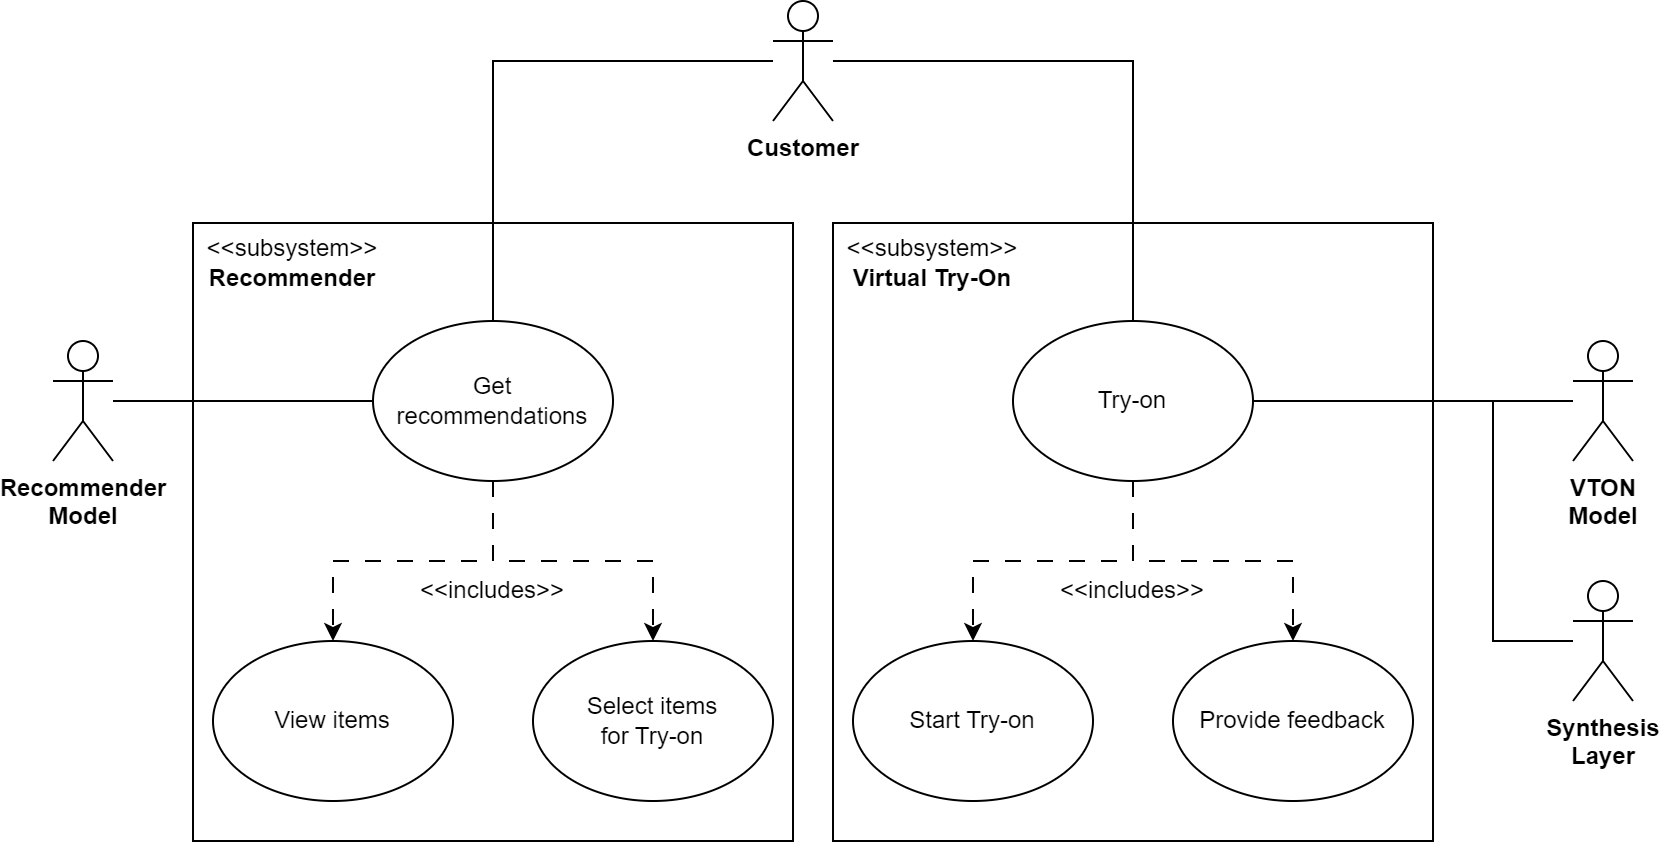
\includegraphics[width=\textwidth]{components/images/use-case.png}
			\caption{Use-case diagram}
			\label{fig:use-case}
		\end{figure}

	\subsection{User Classes and Characteristics}
		The project has the following user classes: 

		\begin{enumerate}
			\item \textbf{Online shoppers:}
				\begin{itemize}
					\item \textit{Characteristics:} Shoppers are the primary end-users of the system. They have varying fashion preferences and seek clothing recommendations that align with their personal style and body type. Shoppers may have different levels of technological proficiency, from tech-savvy individuals to those with limited technology experience.
					\item \textit{Usage:} Shoppers use the system to search for clothing items, receive personalized recommendations, and virtually try on garments. They provide feedback and ratings to refine future recommendations.
				\end{itemize}
			\item \textbf{Retailers and fashion brands:}
				\begin{itemize}
					\item \textit{Characteristics:} Retailers and fashion brands represent business partners or clients who wish to integrate the recommendation and virtual try-on system into their e-commerce platforms. They possess in-depth knowledge of their product catalogs and seek to improve customer engagement and sales.
					\item \textit{Usage:} Retailers and fashion brands collaborate with the development team to integrate the system into their online stores. They may provide fashion catalogs, branding assets, and participate in system customization.
				\end{itemize}
			\item \textbf{Fashion designers and stylists:}
				\begin{itemize}
					\item \textit{Characteristics:} Fashion designers and stylists may collaborate with the system to showcase their clothing collections or styling expertise. They are experts in fashion trends, design, and styling.
					\item \textit{Usage:} Designers and stylists work with retailers to curate clothing collections and styles for the system. They may also provide fashion tips, styling advice, or content to enrich the user experience.
				\end{itemize}
			\item \textbf{Data analysts and AI specialists:}
				\begin{itemize}
					\item \textit{Characteristics:} Data analysts and AI specialists are responsible for fine-tuning the recommendation algorithms and ensuring the system's AI components work optimally. They possess expertise in data analysis and machine learning.
					\item \textit{Usage:} Data analysts and AI specialists continuously improve recommendation algorithms, analyze user data for patterns, and adapt the system to evolving fashion trends and customer preferences.
				\end{itemize}
		\end{enumerate}

\section{Specific Requirements}
	\subsection{Operating Environment}
		The operating environment of our project is as follows:

		\begin{enumerate}
			\item \textbf{Software requirements:}
				\begin{itemize}
					\item \textit{Operating system:} The target end-user operating system may be any of the following platforms which support the ONNX Runtime \cite{onnxruntimeCompatibility}:
						\begin{itemize}
							\item Windows 10 1709+
							\item Linux distributions supported by .NET Core
							\item Mac 10.14+ (Mojave)
							\item Android 28+ (v9 ``Pie")
							\item iOS 12+
						\end{itemize}
					\item \textit{Web browsers:} It should be accessible through popular web browsers like Google Chrome, Mozilla Firefox, Safari, and Microsoft Edge for web-based interfaces.
					\item \textit{AR framework:} A robust AR framework such as AR.js for web-based AR experiences, should be integrated.
					\item \textit{Database management:} The project requires a database management system for user profiles, clothing item information, and preference data. Document-based NoSQL options like Apache Cassandra can be considered.
					\item \textit{Programming languages and libraries:} Development will involve languages like Python and JavaScript, and frameworks like PyTorch and Huggingface Transformers and Optimum for machine learning tasks.
					\item \textit{Machine learning inference:} A cross-platform machine learning runtime like ONNX Runtime which supports the ONNX format, an open standard for machine learning interoperability.
					\item \textit{Web development stack:} For web-based interfaces, a stack including HTML, CSS, JavaScript, and backend frameworks like Node.js and Express will be employed.
				\end{itemize}
			\item \textbf{Hardware requirements:}
			\begin{itemize}
				\item \textit{User devices:} The project is intended to work on a range of user devices like smartphones, tablets, laptops, and desktop computers.
				\item \textit{Cameras and sensors:} Devices should have integrated or attachable cameras and sensors capable of capturing user images and surroundings for the virtual try-on feature.
				\item \textit{CPU:} Any modern multi-core processor with a clock speed of at least 2.5 GHz.
				\item \textit{GPU:}
					\begin{itemize}
						\item Training requirement: A video-card with minimum 8GB VRAM for deep learning tasks.
						\item End-user inference requirement: Any GPU which supports Vulkan APIs.
					\end{itemize}
				\item \textit{Internet connectivity:} A stable internet connection is essential for real-time communication with the server, image processing, and rendering of AR elements.
			\end{itemize}
		\end{enumerate}
	
	\subsection{Design Philosophies}
		\begin{enumerate}
			\item \textbf{User-centric design:} Our design philosophy places the user at the center of the system. We prioritize creating an intuitive and seamless user experience that accommodates users of various demographics and technological backgrounds. User feedback will continuously inform design improvements.
			\item \textbf{Personalization:} The system will employ machine learning algorithms to create a highly personalized experience. User preferences and feedback will be used to tailor clothing recommendations and enhance the virtual try-on experience.
			\item \textbf{Scalability:} The design will be modular and scalable to accommodate a growing user base and evolving technological trends. This approach allows for easy integration of new features and accommodates increased usage loads.
			\item \textbf{Security and privacy:} Security and privacy will be fundamental to the design, with strong encryption protocols for data protection. Users' personal information and imagery will be handled with the utmost care, and adherence to data protection regulations is a priority.
		\end{enumerate}

	\subsection{Implementation Philosophies}
		\begin{enumerate}
			\item \textbf{State-of-the-Art AI:} Implementation will involve integrating state-of-the-art machine learning and computer vision techniques to ensure accurate clothing recommendations and realistic virtual try-on experiences. We will employ libraries and frameworks with active development and community support.
			\item \textbf{Cross-platform compatibility:} The system will be developed with cross platform compatibility in mind. Web interfaces will be developed to ensure that users can access and utilize the system seamlessly on various devices.
			\item \textbf{Continuous testing and iteration:} Agile development methodologies will be used to enable continuous testing, feedback, and iteration. This approach allows us to respond to user needs, refine algorithms, and enhance system performance throughout development.
		\end{enumerate}

	\subsection{Constraints}
		\begin{enumerate}
			\item \textbf{Data Privacy and Compliance:} The project must adhere to strict data privacy regulations. This imposes constraints on how user data is collected, stored, and utilized.
			\item \textbf{Resource Limitations:} The project will operate within resource constraints, including budget and available hardware resources, which may affect the system's scalability and performance.
			\item \textbf{Technological Compatibility:} The system must work across a wide range of devices and platforms, which presents constraints related to compatibility and performance optimization.
			\item \textbf{User Connectivity:} User experience may be affected by the quality of the user's internet connection, especially when utilizing the augmented reality feature. Ensuring a functional experience even in low-bandwidth situations is a constraint.
		\end{enumerate}

\section{External Interface Requirements}
	\subsection{User Interfaces}
		The primary user interface will be web-based and accessible via standard web browsers. It should be compatible with popular web browsers, including but not limited to Google Chrome, Mozilla Firefox, Microsoft Edge, and Safari. The user interface should be responsive, adapting to various screen sizes, including desktops, tablets, and mobile devices.

		The virtual try-on interface relies on AR and should be compatible with most devices. It must support features such as real-time clothing overlay and interactive controls for users to try on clothing items seamlessly.
	
	\subsection{Hardware Interfaces}
		The virtual try-on feature requires the use of cameras and sensors. Our system should interface with these devices to capture images and detect user movements for an immersive AR experience. These interfaces should be compatible with a range of devices.

	\subsection{Software Interfaces}
		\subsubsection{Clothing Recommendation Interface}
			The system will interface with a clothing recommendation algorithm to leverage advanced recommendation algorithms for personalized clothing suggestions.

			Requirements:
			\begin{enumerate}
				\item The system should send user profile and preferences data to the recommendation algorithm.
				\item The algorithm should return a list of recommended clothing items.
				\item The interface should allow for updates to the recommendation algorithm without affecting core system functionality.
			\end{enumerate}
		
		\subsubsection{AR Virtual Try-On Interface}
			The system will interface with an AR module for virtual clothing try-on to enable users to visualize clothing items on themselves in real-time.

			Requirements:
			\begin{enumerate}
				\item The AR module must support 3D model rendering of clothing items on user images.
				\item It should provide accurate real-time visualization.
				\item The system should send data about selected clothing items to the AR module for rendering.
				\item The AR module should return rendered images or video streams of users with clothing items superimposed.
			\end{enumerate}

		\subsubsection{User Profile and Preferences Data Interface}
			The system will interact with user profile and preferences data to gather information about user preferences and characteristics for clothing recommendations.

			Requirements:
			\begin{enumerate}
				\item The system must allow users to create and update their profiles.
				\item It should securely store and retrieve user data.
				\item The interface must be compliant with data protection regulations.
			\end{enumerate}

\section{Other Nonfunctional Requirements}
	\subsection{Performance Requirements}
		The system should be able to read and understand the human body and be able to parse the areas of interests, generate outfit accordingly and finally, render the subject in real-time through augmented reality.
		
		\subsubsection{Resource utilization}
			For the system to be compatible with majority devices including low powered mobiles and tablets, the resource utilization should be kept to minimum without affecting the quality of output.

		\subsubsection{Feedback duration}
			As expected of the try-on systems, the system should be able to provide feedback on the subject in real-time. Processing time should be kept as low as possible for better experience for user.

		\subsubsection{Feedback quality}
			The system should generate personalized outfit and the subject should be able to judge the proposed style and size on itself. The process should be both convenient and rewarding for the user.
		
	\subsection{Safety and Security Requirements}
		\begin{enumerate}
			\item \textbf{Privacy compliance:} The user shouldn't be concerned about disclosure of his/her features to open userbase. The system should only parse the regions of interest for building the metrics of generation and should not intent to perform any malicious operations.
			\item \textbf{Ethics:} The system should not delve into inappropriate outfit generation and should take into account of user's modesty. The system shouldn't be biased towards certain age groups, races or color.
			\item \textbf{Compliances:} The system should adhere to rules and compliances stated by the authorities and stakeholders and should limit it's working domain to that specified be the compliances.
		\end{enumerate}
	
	\subsection{Acceptance Criteria}
		Give the scenario where the user has selected certain clothes according to their preferences and is expecting the system to generate the outfit on their body so that they can judge the style and the overall look of the outfit, the user lets the camera record their body. Both the subject body features and generated recommendations are input for the system.

		When the user selects generate outfit option after selection of styles recommended or chosen by himself/herself. The system segments the features from the subject and tries to wrap the outfit around them. If the system is well trained on personalized recommendation and virtual try-on, the system successfully generates the outfit personalized to the subject and provides the rendered view in augmented reality.

	\subsection{Software Quality Attributes}
		\begin{enumerate}
			\item \textbf{Reliability:} The system should be dependable, providing accurate clothing recommendations and ensuring that the virtual try-on feature functions consistently without errors or crashes.
			\item \textbf{Usability:} User interfaces should be intuitive and user-friendly, making it easy for customers to navigate the system and obtain clothing suggestions effortlessly.
			\item \textbf{Maintainability:} The codebase should be well-organized, documented, and structured to facilitate updates, enhancements, and bug fixes.
			\item \textbf{Flexibility:} The system should adapt to changes in user preferences, allowing for the integration of new fashion items and the modification of recommendation algorithms.
			\item \textbf{Robustness:} The system should be able to handle unexpected inputs or situations without crashing or providing inaccurate results.
		\end{enumerate}

\section{Future Scope}
	The project opens up the following future developments:

	\begin{enumerate}
		\item Inclusion of more body types.
		\item Extended clothing categories and varieties.
		\item Multi-modal integration such as voice-activated commands and gesture-based interactions for enhanced virtual try-ons.
		\item Integration of social media elements.
		\item Integration with wearable technology.
		\item Fashion trend analysis and prediction to aide recommendations.
	\end{enumerate}
	\chapter[Algorithm Analysis \& Mathematical Modeling]{ALGORITHM ANALYSIS \& MATHEMATICAL MODELING}

\section{Convolutional Neural Networks}
	CNNs play a crucial role in this project, specifically in enhancing the analysis and understanding of clothing images and the user's body. They can be used for the following tasks:

	\begin{enumerate}
		\item \textbf{Visual analysis of clothing items:} CNNs are employed to analyze and extract visual features from images of clothing items. This process enables the system to understand the style, design, color, and other visual attributes of each garment.
		\item \textbf{Feature extraction:} CNNs extract high-level features from clothing images, allowing the system to identify patterns, textures, and details in the garments. This feature extraction aids in the matching of user preferences with visually similar items. Further, they can be used for feature extraction from the user's image, to learn about body attributes.
		\item \textbf{Visual compatibility assessment:} CNNs can be utilized to assess the visual compatibility of clothing combinations, helping users put together stylish outfits. This ensures that the virtual try-on experience reflects real-world fashion sensibilities.
	\end{enumerate}

\section{Matrix Factorization}
	Matrix factorization is a fundamental technique employed to model user-item interactions, extract latent factors, and generate personalized clothing recommendations. In this context, matrix factorization primarily focuses on the following aspects:

	\begin{enumerate}
		\item \textbf{User-item interaction matrix:} A user-item interaction matrix is constructed with users represented along one axis, and clothing items along the other axis. This matrix captures the historical interactions of users with clothing items, such as views, clicks, purchases, and preferences.
		\item \textbf{Latent factor discovery:} Matrix factorization techniques are applied to decompose the user-item interaction matrix into two lower-dimensional matrices, one representing users' latent factors and the other representing items' latent factors. These latent factors capture unobservable characteristics of both users and clothing items. Users with similar tastes have similar latent factors, and clothing items with similar attributes have similar latent factors.
		\item \textbf{Recommendation generation:} Once the latent factors are discovered, a recommendation engine can employ them to generate personalized recommendations. This is achieved by estimating missing entries in the interaction matrix, indicating which clothing items a user may be interested in. The engine ranks items based on these estimates and presents the top recommendations to the user.
	\end{enumerate}

\section{Bayesian Personalized Ranking}
	BPR addresses a critical challenge in the realm of fashion e-commerce. It is used to optimize the ranking of clothing items within our recommendation system, ensuring that users are presented with items that align closely with their preferences and style. Here's how BPR can be applied:

	\begin{enumerate}
		\item \textbf{Personalized ranking:} BPR focuses on the individual preferences and interactions of users. It acknowledges that each user has unique tastes and that the success of a recommendation system lies in its ability to rank items according to these individual preferences.
		\item \textbf{Implicit feedback:} BPR is particularly well-suited for scenarios where implicit feedback is abundant. In the fashion e-commerce domain, user interactions are often implicit, including clicks, views, and purchases. BPR leverages these implicit signals to understand user preferences, creating a ranking of items based on the likelihood of user engagement.
	\end{enumerate}

\section{Siamese Networks and Triplet Loss}
	Siamese Networks and triplet loss emerge as essential tools for enhancing the accuracy and quality of the recommendation and virtual try-on systems.

	\subsection*{Siamese Networks}
		Siamese networks are fundamental for both the recommendation engine and virtual try-on systems. They can be employed to measure the similarity between user preferences and clothing items. By learning similarity metrics, the recommendation system can identify items that align with a user's unique style. Siamese networks enhance the ability to create personalized recommendations by assessing the closeness of user preferences and clothing features. In the virtual try-on system, Siamese networks play a pivotal role in assessing how well a selected clothing item fits and matches the user's style. By comparing the virtual try-on with the user's image, the network can provide real-time feedback on the fit, style, and overall suitability of the item.

	\subsection*{Triplet Loss}
		Triplet loss can be used to create embeddings for clothing items, user profiles, and the user's virtual try-on. By learning triplets composed of an anchor item (selected clothing item), a positive item (a similar item that the user may like), and a negative item (a dissimilar item), the network can generate embeddings that capture the nuances of user preferences. This enables the system to recommend items that closely match the user's style and improve the virtual try-on experience.

	The focus is on creating robust embeddings and similarity metrics. The network contributes to the project's core objectives of providing personalized clothing recommendations and an immersive virtual try-on experience, ultimately enhancing user engagement and satisfaction in online fashion retail.

\section{Transformers}
	Transformers, originally developed for natural language processing tasks, have proven to be versatile and valuable in various domains, including computer vision and recommendation systems. Transformers can be utilized in the following ways:

	\begin{enumerate}
		\item \textbf{Textual data analysis:} Transformers can be used to analyze textual data associated with clothing items, such as product descriptions, customer reviews, and style attributes. By understanding the semantics and context of these descriptions, Transformers enhance the recommendation system's ability to capture the fine-grained details of clothing items.
		\item \textbf{Multimodal representations:} Transformers are used to create multimodal embeddings that relate both textual and visual features of clothing items. These embeddings capture a holistic view of fashion items by integrating information from both text and images. The resulting embeddings are valuable for recommendation accuracy.
		\item \textbf{Image synthesis enhancement:} In the virtual try-on component, Transformers help in image recognition, style matching, and visual understanding. They optimize the overlay of digital clothing items on users' images, ensuring a realistic and visually appealing virtual try-on experience.
	\end{enumerate}

\section{PseudoCode}
\subsection{Fashion Recommendation}
\BlankLine
\begin{algorithm}[H]
  \SetAlgoLined
  \SetKwInOut{Input}{Input}
  \SetKwInOut{Output}{Output}

  \Input{user\_data}
  \Output{preprocessed user\_data}

  \caption{Preprocess User Data}
  \label{alg:preprocess_user_data}
  \BlankLine

  \SetKwFunction{FMain}{preprocess\_user\_data}
  \SetKwProg{Fn}{Function}{:}{}
  \Fn{\FMain{data}}{
    cleaned\_data = handle\_missing\_values(data)\;
    encoded\_data = encode\_categorical\_data(cleaned\_data)\;
    normalized\_data = normalize\_numerical\_data(encoded\_data)\;
    \KwRet normalized\_data\;
  }
\end{algorithm}
 \BlankLine
Preprocess User data:
 \BlankLine
\begin{itemize}
\item This function cleans and prepares user data for further processing.
\item It handles missing values by imputing them with appropriate strategies like mean or median.
\item Categorical data (e.g., user preferences like color, style) is converted into numerical representation (e.g., one-hot encoding).
\item Numerical data (e.g., user demographics like age) is normalized to a common scale for better comparison.
\end{itemize}
 \BlankLine

\begin{algorithm}[H]
  \SetAlgoLined
  \SetKwInOut{Input}{Input}
  \SetKwInOut{Output}{Output}

  \Input{clothing\_data}
  \Output{preprocessed clothing\_data}

  \caption{Preprocess Clothing Data}
  \label{alg:preprocess_clothing_data}
  \BlankLine

  \SetKwFunction{FMain}{preprocess\_clothing\_data}
  \SetKwProg{Fn}{Function}{:}{}
  \Fn{\FMain{data}}{
    resized\_data = resize\_images(data)\;
    resnet\_ready\_data = preprocess\_for\_resnet(resized\_data)\;
    \KwRet resnet\_ready\_data\;
  }
\end{algorithm}
 \BlankLine
Preprocess Clothing data:
 \BlankLine
\begin{itemize}
    \item This function prepares clothing data, likely consisting of images, for feature extraction.
    \item Images might be resized to a standard size to ensure consistent processing by the ResNet50 model.
    \item Additional preprocessing steps might be necessary depending on the specific model requirements (e.g., color normalization, mean subtraction).
\end{itemize}
 \BlankLine
\begin{algorithm}[H]
  \SetAlgoLined
  \SetKwInOut{Input}{Input}
  \SetKwInOut{Output}{Output}

  \Input{data}
  \Output{features}

  \caption{Extract Features using ResNet50}
  \label{alg:extract_features_resnet}
  \BlankLine

  \SetKwFunction{FMain}{extract\_features\_resnet}
  \SetKwProg{Fn}{Function}{:}{}
  \Fn{\FMain{data}}{
    resnet\_model = load\_resnet\_model()\;
    features = resnet\_model.predict(data)\;
    \KwRet features\;
  }
\end{algorithm}
 \BlankLine
Extract Features Resnet:
 \BlankLine
\begin{itemize}
    \item This function utilizes a pre-trained ResNet50 model for feature extraction.
    \item The ResNet50 model, a deep learning architecture, is used to capture high-level features from both user and clothing data.
    \item These features represent essential characteristics of the data, allowing for comparison between user preferences and clothing items.
\end{itemize}
 \BlankLine
\begin{algorithm}[H]
  \SetAlgoLined
  \SetKwInOut{Input}{Input}
  \SetKwInOut{Output}{Output}

  \Input{user\_features, clothing\_features}
  \Output{k nearest neighbors}

  \caption{Find Nearest Neighbors}
  \label{alg:find_nearest_neighbors}
  \BlankLine

  \SetKwFunction{FMain}{find\_nearest\_neighbors}
  \SetKwProg{Fn}{Function}{:}{}
  \Fn{\FMain{user\_features, clothing\_features, k}}{
    distances = calculate\_pairwise\_distances(user\_features, clothing\_features)\;
    nearest\_neighbors = identify\_k\_nearest\_neighbors(distances, k)\;
    \KwRet nearest\_neighbors\;
  }
\end{algorithm}
 \BlankLine
Find Nearest Neighbors:
 \BlankLine
\begin{itemize}
    \item This function identifies the k nearest neighbors (clothing items) for a given user.
    \item It calculates the distance (similarity) between the user's features and the features of each clothing item. This distance metric could be Euclidean distance for numerical features.
    \item Based on the calculated distances, the function identifies the k clothing items with the most similar features, representing potential recommendations for the user.
\end{itemize}
 \BlankLine
\begin{algorithm}[H]
  \SetAlgoLined
  \SetKwInOut{Input}{Input}
  \SetKwInOut{Output}{Output}

  \Input{recommendations, user\_preferences, ratings}
  \Output{refined recommendations}

  \caption{Refine Recommendations}
  \label{alg:refine_recommendations}
  \BlankLine

  \SetKwFunction{FMain}{refine\_recommendations}
  \SetKwProg{Fn}{Function}{:}{}
  \Fn{\FMain{recommendations, user\_preferences, ratings}}{
    weighted\_recommendations = apply\_preference\_weights(recommendations, user\_preferences)\;
    refined\_recommendations = incorporate\_ratings(weighted\_recommendations, ratings)\;
    \KwRet refined\_recommendations\;
  }
\end{algorithm}
 \BlankLine
Refine Recommendations:
 \BlankLine
\begin{itemize}
    \item This function takes the initial recommendations (k nearest neighbors) and refines them based on user preferences and ratings.
    \item User preferences (e.g., preferred styles, colors) are retrieved from the user data.
    \item Weights are applied to the recommendations, giving higher priority to items that match user preferences.
    \item The function might incorporate collaborative filtering by considering user ratings on similar items, potentially recommending items that other users with similar preferences have rated highly.
     \BlankLine
\end{itemize}
\subsection{AIR-VTON}
\begin{algorithm}[H]
  \SetAlgoLined
  \SetKwInOut{Input}{Input}
  \SetKwInOut{Output}{Output}

  \Input{person\_image, clothing\_image}
  \Output{preprocessed person\_image, preprocessed clothing\_image}

  \caption{Preprocessing}
  \label{alg:preprocess}
  \BlankLine

  \SetKwFunction{FMain}{preprocess}
  \SetKwProg{Fn}{Function}{:}{}
  \Fn{\FMain{image}}{
    resized\_image = resize(image)\;
    normalized\_image = normalize(resized\_image)\;
    \KwRet normalized\_image\;
  }
\end{algorithm}
\BlankLine
Preprocessing:
\BlankLine
\begin{itemize}
    \item Resizes the input image to a fixed size, ensuring compatibility with the model.
    \item Normalizes pixel values (often to a range of 0 to 1), preparing them for the neural network.
    \item Returns the preprocessed image.
\end{itemize}


\BlankLine

\begin{algorithm}[H]
  \SetAlgoLined
  \SetKwInOut{Input}{Input}
  \SetKwInOut{Output}{Output}

  \Input{image}
  \Output{body keypoints}

  \caption{Pose Estimation}
  \label{alg:pose_estimation}
  \BlankLine

  \SetKwFunction{FMain}{pose\_estimation}
  \SetKwProg{Fn}{Function}{:}{}
  \Fn{\FMain{image}}{
    preprocessed\_image = preprocess(image)\;
    pose\_model = cv2.dnn.readNetFromModelZoo("path/to/pose\_model.pb", "path/to/pose\_config.pbtxt")\;
    pose\_result = pose\_model.forward(preprocessed\_image)\;
    body\_keypoints = pose\_model.extract(features)\;
    \KwRet body\_keypoints\;
  }
\end{algorithm}
\BlankLine
Pose Estimation:

\begin{itemize}
    \item Preprocesses the image for the specific pose estimation model being used.
    \item Loads a pre-trained pose estimation model (like OpenPose or AlphaPose).
    \item Performs pose estimation using the loaded model to identify body keypoints.
    \item Extracts the body pose keypoints from the model's output.
    \item Returns the extracted body pose keypoints.
\end{itemize}
\BlankLine
\begin{algorithm}[H]
  \SetAlgoLined
  \SetKwInOut{Input}{Input}
  \SetKwInOut{Output}{Output}

  \Input{person\_image, clothing\_image}
  \Output{combined\_features}

  \caption{Encoder Network}
  \label{alg:encoder}
  \BlankLine

  \SetKwFunction{FMain}{encoder}
  \SetKwProg{Fn}{Function}{:}{}
  \Fn{\FMain{person\_image, clothing\_image}}{
    person\_features = cnn\_encoder(person\_image)\;
    clothing\_features = cnn\_encoder(clothing\_image)\;
    combined\_features = combine(person\_features, clothing\_features)\;
    \KwRet combined\_features\;
  }
\end{algorithm}
\BlankLine
Encoder Network:
\BlankLine
\begin{itemize}
    \item Uses a Convolutional Neural Network (CNN) with multiple layers.
    \item Extracts features from the person image and clothing image using the CNN.
    \item Combines the extracted person and clothing features (e.g., by concatenation).
    \item Returns the combined features.
\end{itemize}
\BlankLine

\begin{algorithm}[H]
  \SetAlgoLined
  \SetKwInOut{Input}{Input}
  \SetKwInOut{Output}{Output}

  \Input{combined\_features}
  \Output{warped\_clothing\_features, segmentation\_mask}

  \caption{Decoder Network}
  \label{alg:decoder}
  \BlankLine

  \SetKwFunction{FMain}{decoder}
  \SetKwProg{Fn}{Function}{:}{}
  \Fn{\FMain{combined\_features}}{
    warped\_clothing\_features = decoder\_block(combined\_features, upsample=True)\;
    segmentation\_mask = segmentation\_head(combined\_features)\;
    \KwRet warped\_clothing\_features, segmentation\_mask\;
  }
\end{algorithm}
\BlankLine
Decoder Network
\BlankLine
\begin{itemize}
    \item Takes the combined features from the encoder.
    \item Uses a series of convolutional layers with upsampling to increase the resolution.
    \item Generates warped clothing features: These features describe how the clothing should be deformed to fit the person's body.
    \item Uses a convolutional layer to predict a segmentation mask. This mask identifies which pixels belong to the person in the final image.
    \item Returns the warped clothing features and the segmentation mask.
\end{itemize}
\BlankLine
\begin{algorithm}[H]
  \SetAlgoLined
  \SetKwInOut{Input}{Input}
  \SetKwInOut{Output}{Output}

  \Input{clothing\_image, warped\_features}
  \Output{warped\_clothing}

  \caption{Warp Clothing Image}
  \label{alg:warp_image}
  \BlankLine

  \SetKwFunction{FMain}{warp\_image}
  \SetKwProg{Fn}{Function}{:}{}
  \Fn{\FMain{clothing\_image, warped\_features}}{
    deformation\_grid = generate\_deformation\_grid(warped\_features)\;
    warped\_clothing = warp(clothing\_image, deformation\_grid)\;
    \KwRet warped\_clothing\;
  }
\end{algorithm}
\BlankLine
Warp Clothing Image
\BlankLine
\begin{itemize}
    \item Takes the clothing image and the warped features from the decoder.
    \item Uses the warped features to create a deformation grid.
    \item This grid defines how to warp the clothing image to fit the person's body shape.
    \item Warps the clothing image using the deformation grid.
    \item Returns the warped clothing image.
\end{itemize}
\BlankLine

\begin{algorithm}[H]
  \SetAlgoLined
  \SetKwInOut{Input}{Input}
  \SetKwInOut{Output}{Output}

  \Input{person\_image, warped\_clothing, segmentation\_mask}
  \Output{final\_image}

  \caption{Image Fusion}
  \label{alg:image_fusion}
  \BlankLine

  \SetKwFunction{FMain}{combine\_images}
  \SetKwProg{Fn}{Function}{:}{}
  \Fn{\FMain{person\_image, warped\_clothing, segmentation\_mask}}{
    person\_mask = 1 - segmentation\_mask\;
    person\_region = person\_image * person\_mask\;
    final\_image = warped\_clothing * segmentation\_mask + person\_region\;
    \KwRet final\_image\;
  }
\end{algorithm}
\BlankLine
Image Fusion
\BlankLine
\begin{itemize}
    \item Takes the person image, the warped clothing, and the segmentation mask.
    \item Creates a person mask by inverting the segmentation mask (isolating the person region).
    \item Extracts the person region from the original image using the person mask.
    \item Combines the warped clothing with the person region based on the segmentation mask.
    \item This ensures realistic placement of the clothing on the person's body.
    \item Returns the final image with the virtual try-on effect.
\end{itemize}
	\chapter[Detailed Design]{DETAILED DESIGN}

\section{Architectural Design}
	\begin{figure}[h!]
		\centering
		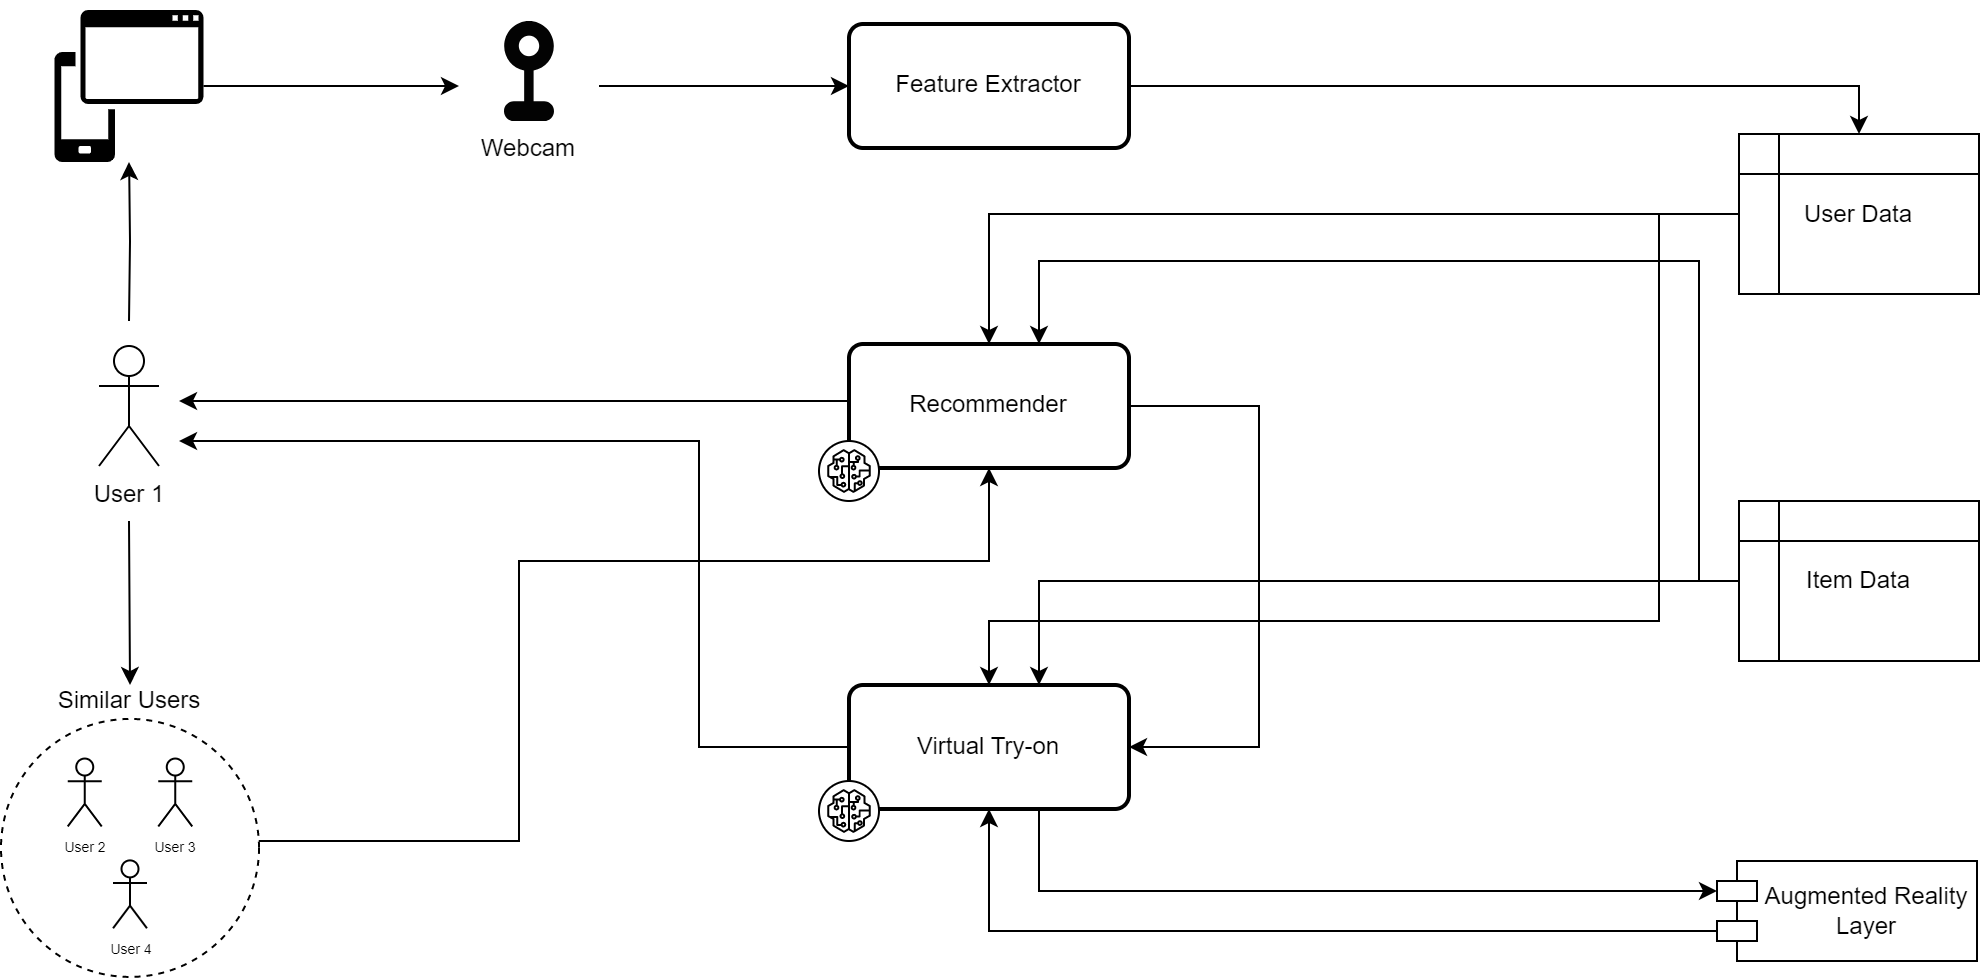
\includegraphics[width=0.75\textwidth]{components/images/sys-arch.png}
		\caption{System Architecture}
		\label{fig:sys-arch}
	\end{figure}

\section{UML Diagrams}
	\subsection{Use-case Diagram}
		\begin{figure}[h!]
			\centering
			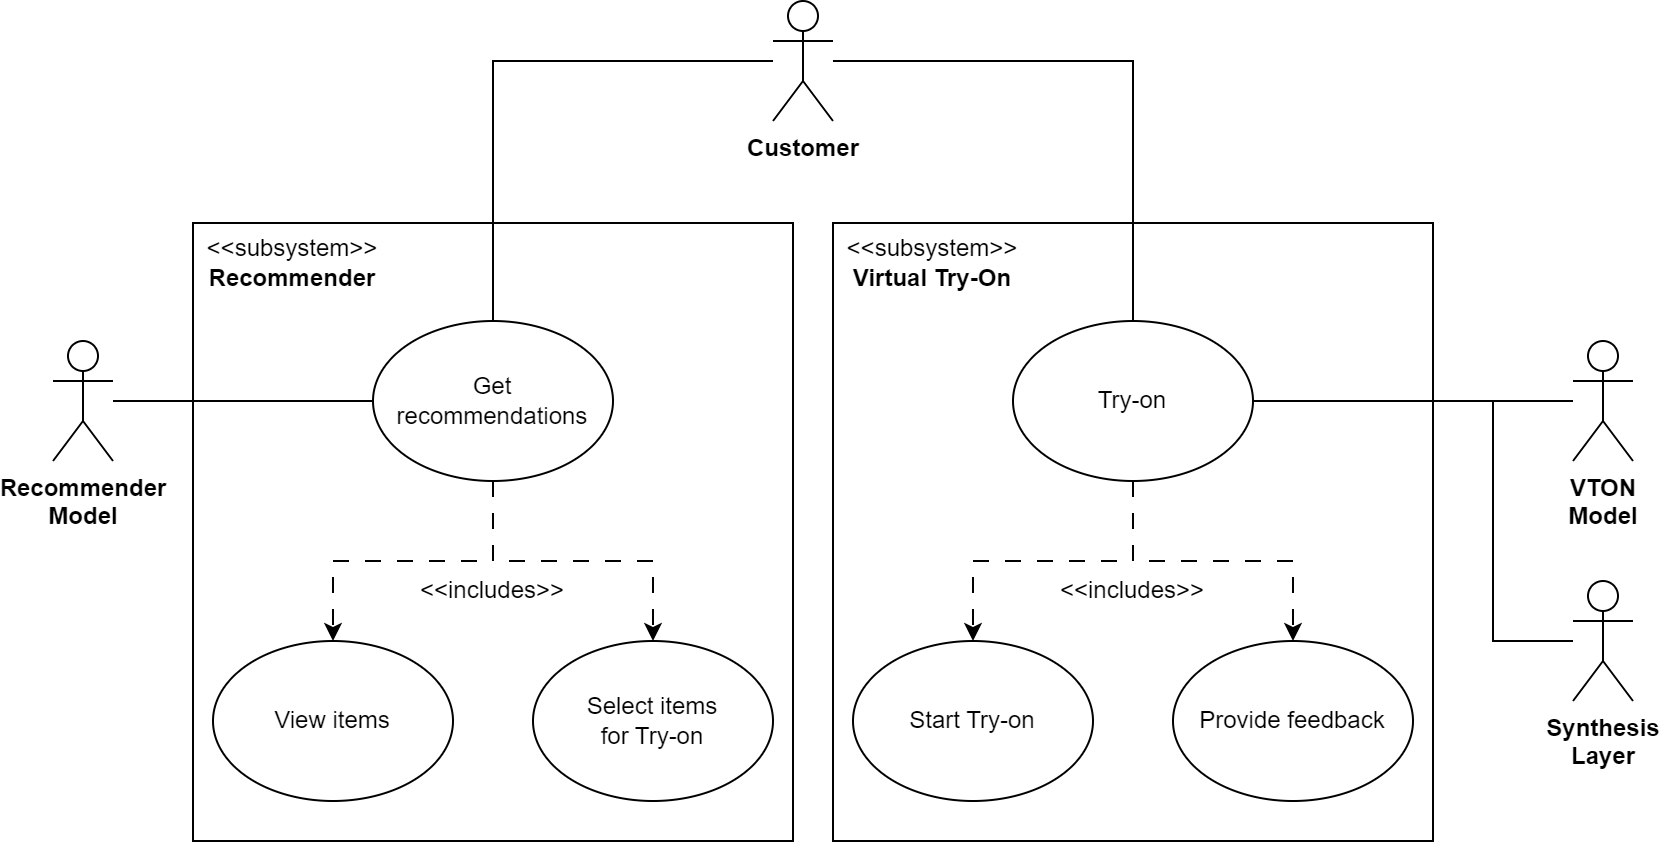
\includegraphics[width=0.75\textwidth]{components/images/use-case.png}
			\caption{Use-case Diagram}
			\label{fig:use-case-rep}
		\end{figure}

	\pagebreak

	\subsection{Sequence Diagram}
		\begin{figure}[h!]
			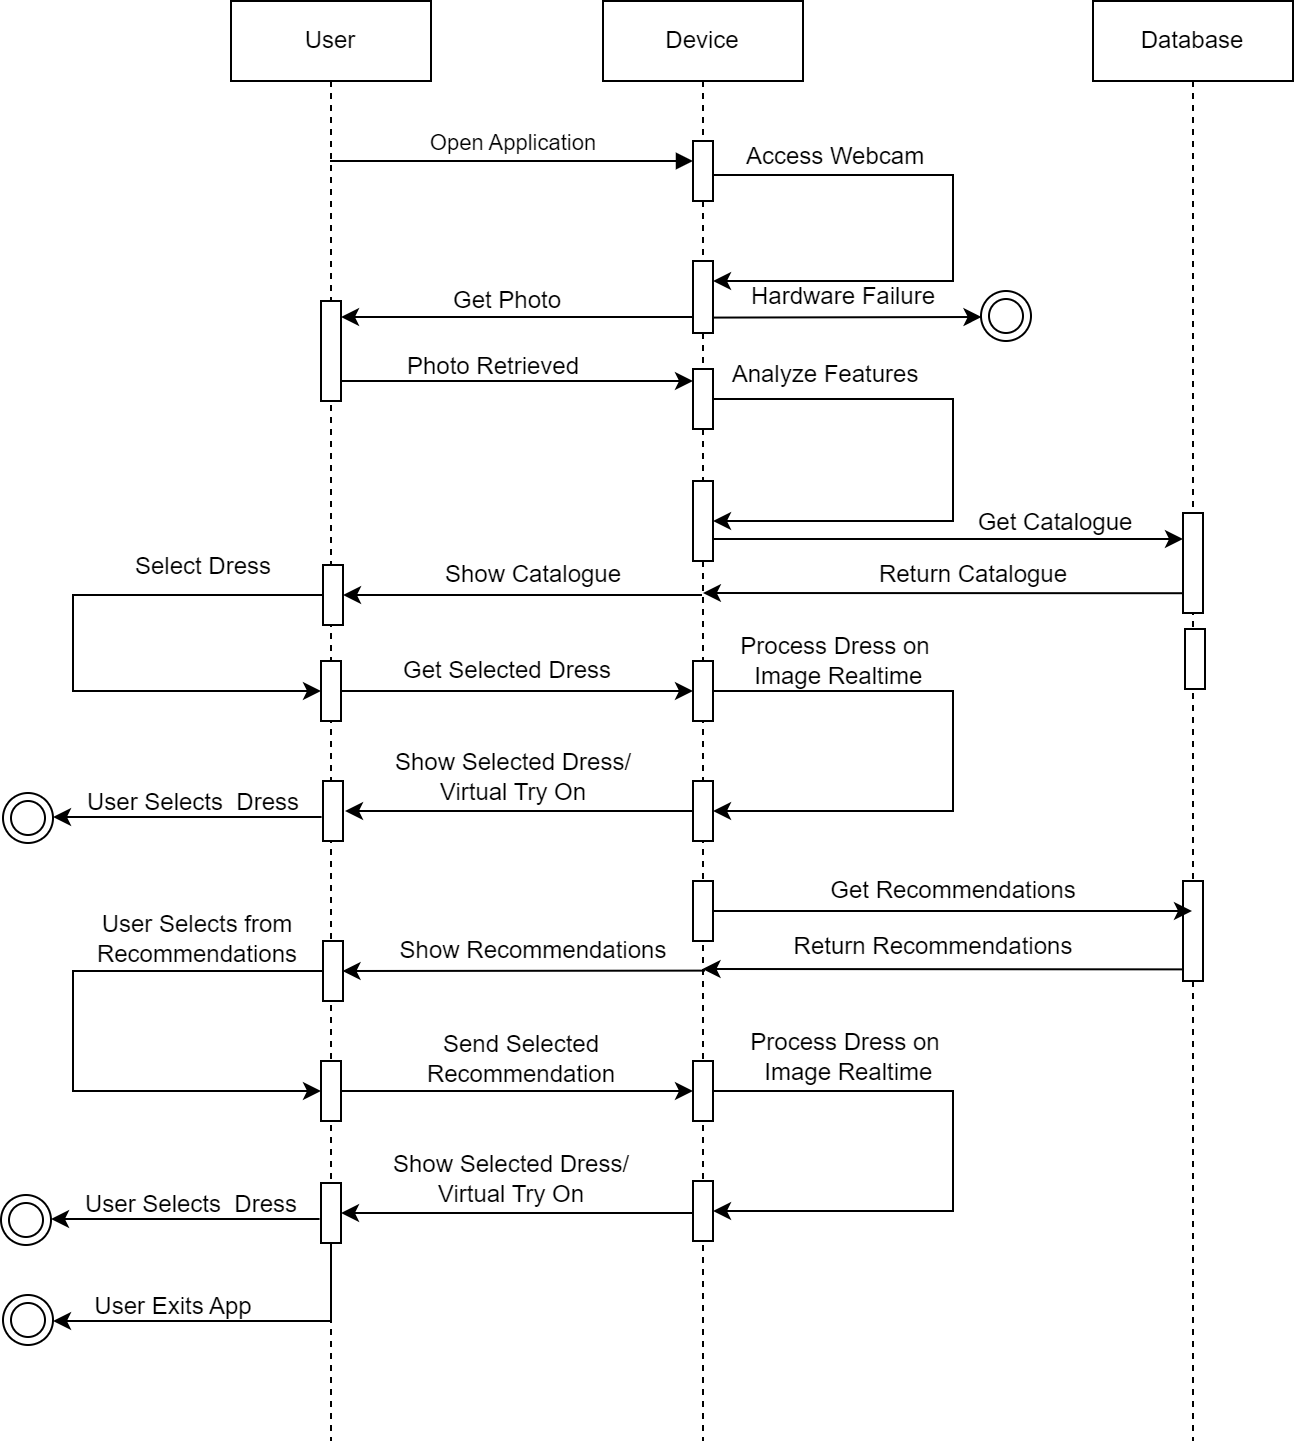
\includegraphics[width=\textwidth]{components/images/sequence.png}
			\caption{Sequence Diagram}
			\label{fig:sequence}
		\end{figure}

	\pagebreak

	\subsection{Activity Diagram}
		\begin{figure}[h!]
			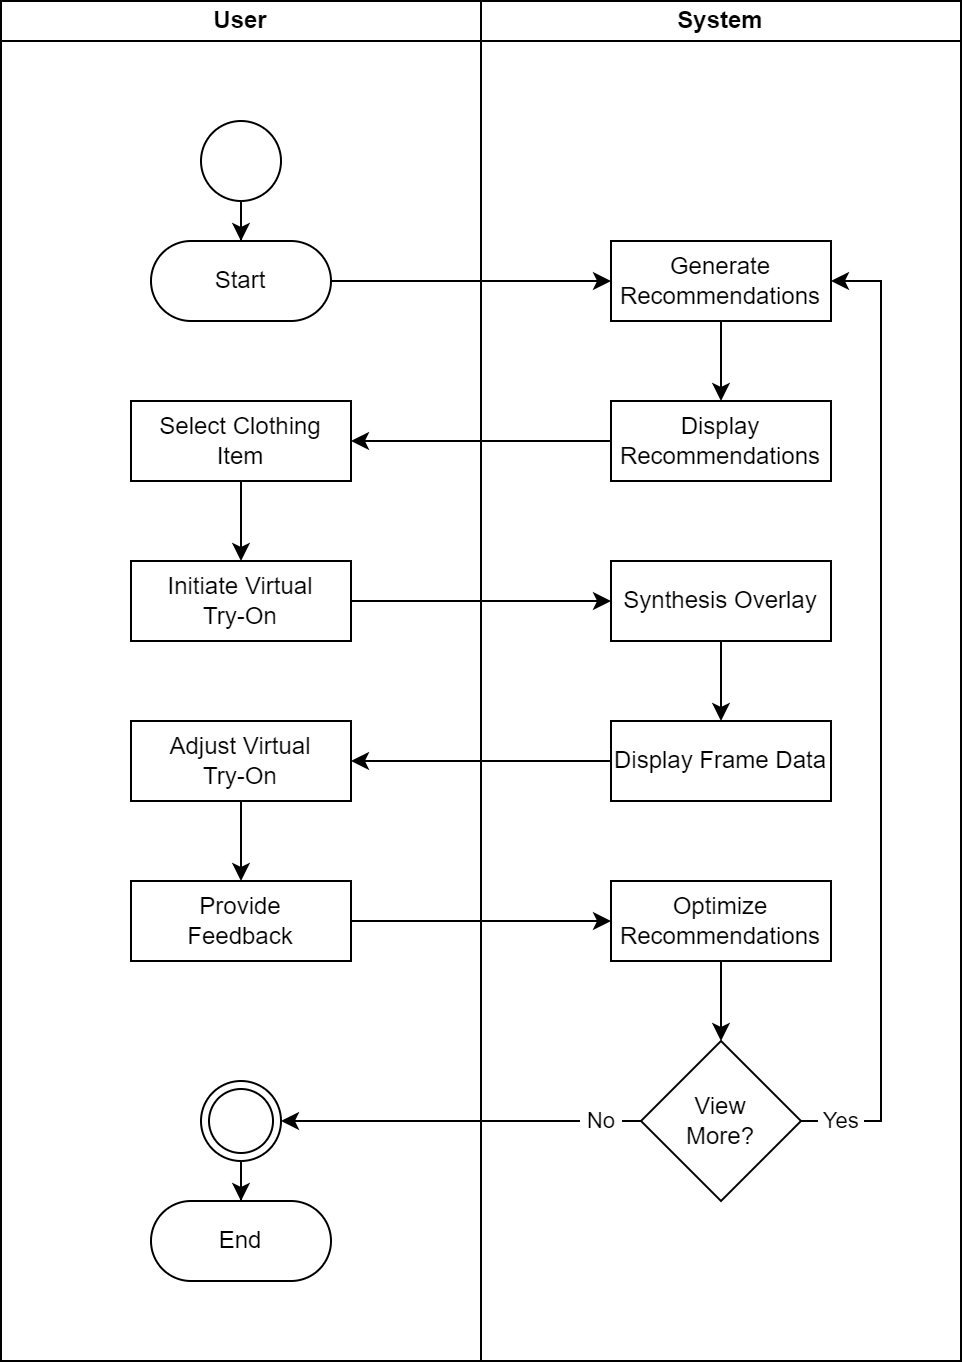
\includegraphics[width=\textwidth]{components/images/activity.png}
			\caption{Activity Diagram}
			\label{fig:activity}
		\end{figure}

	\pagebreak

	\subsection{State Diagram}
		\begin{figure}[h!]
			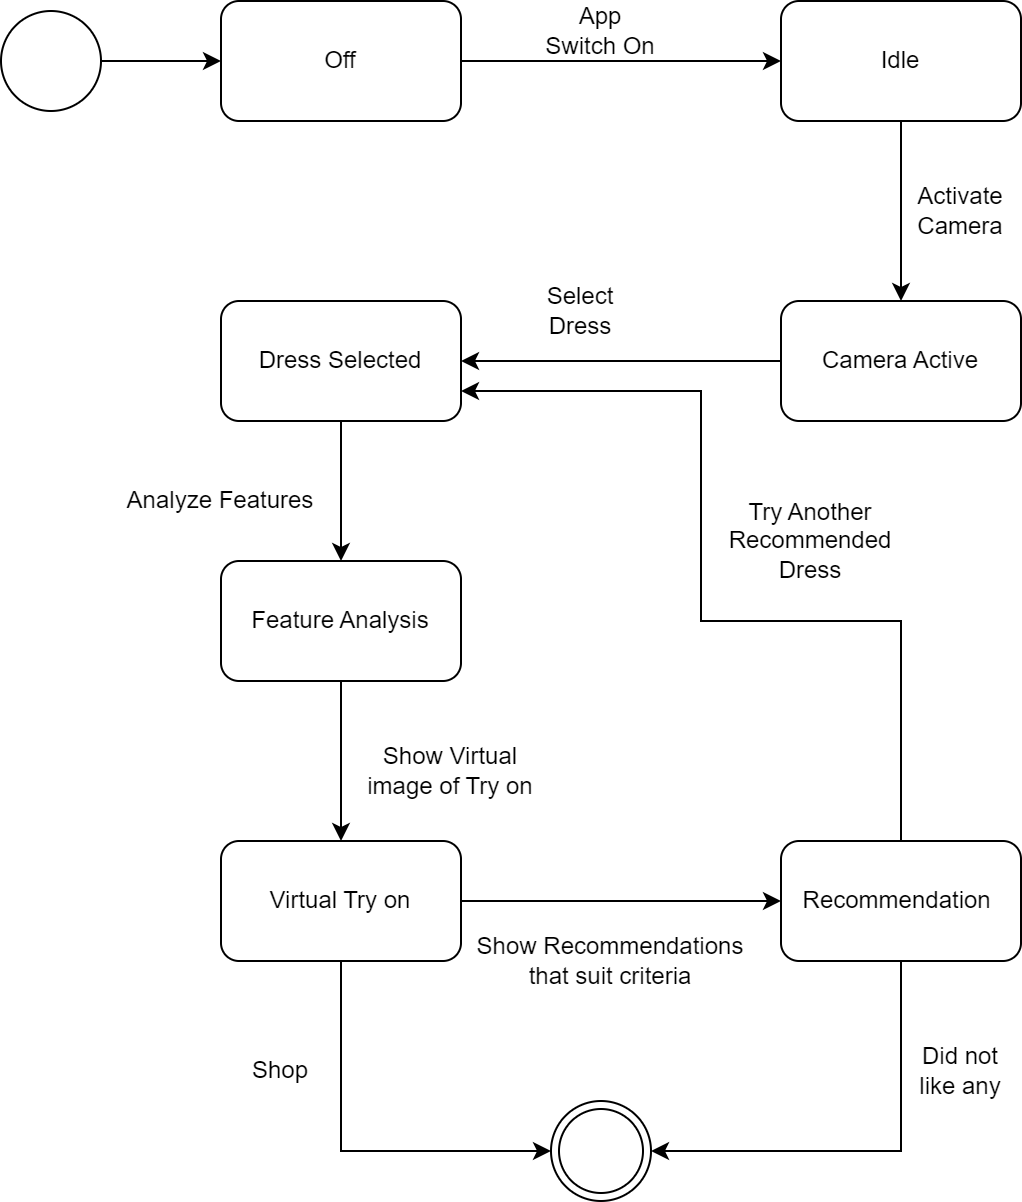
\includegraphics[width=\textwidth]{components/images/state.png}
			\caption{State Diagram}
			\label{fig:state}
		\end{figure}

	\pagebreak

	\subsection{Component Diagram}
		\begin{figure}[h!]
			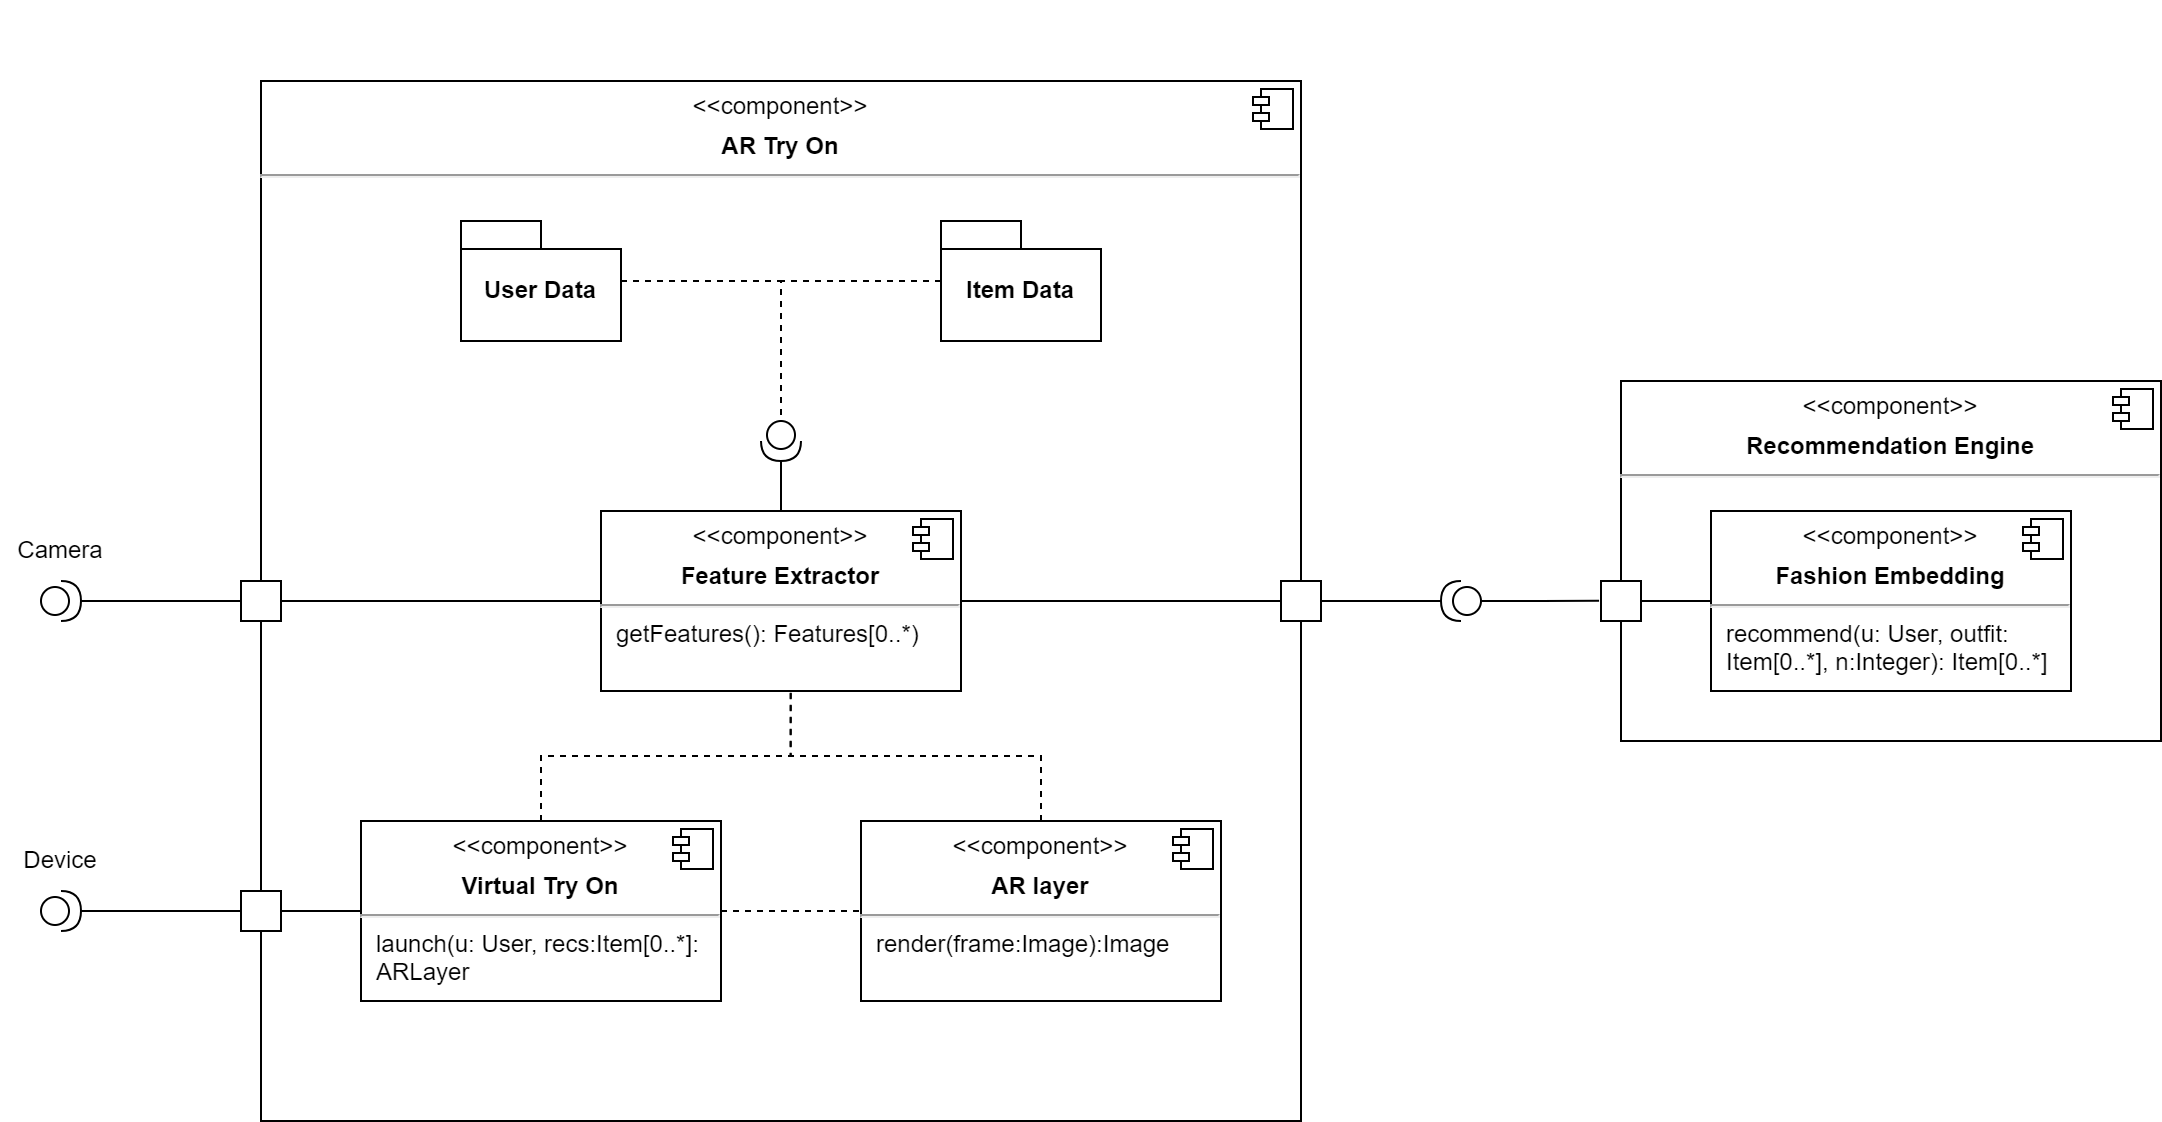
\includegraphics[width=\textwidth]{components/images/component.png}
			\caption{Component Diagram}
			\label{fig:component}
		\end{figure}

	\subsection{Class Diagram}
		\begin{figure}[h!]
			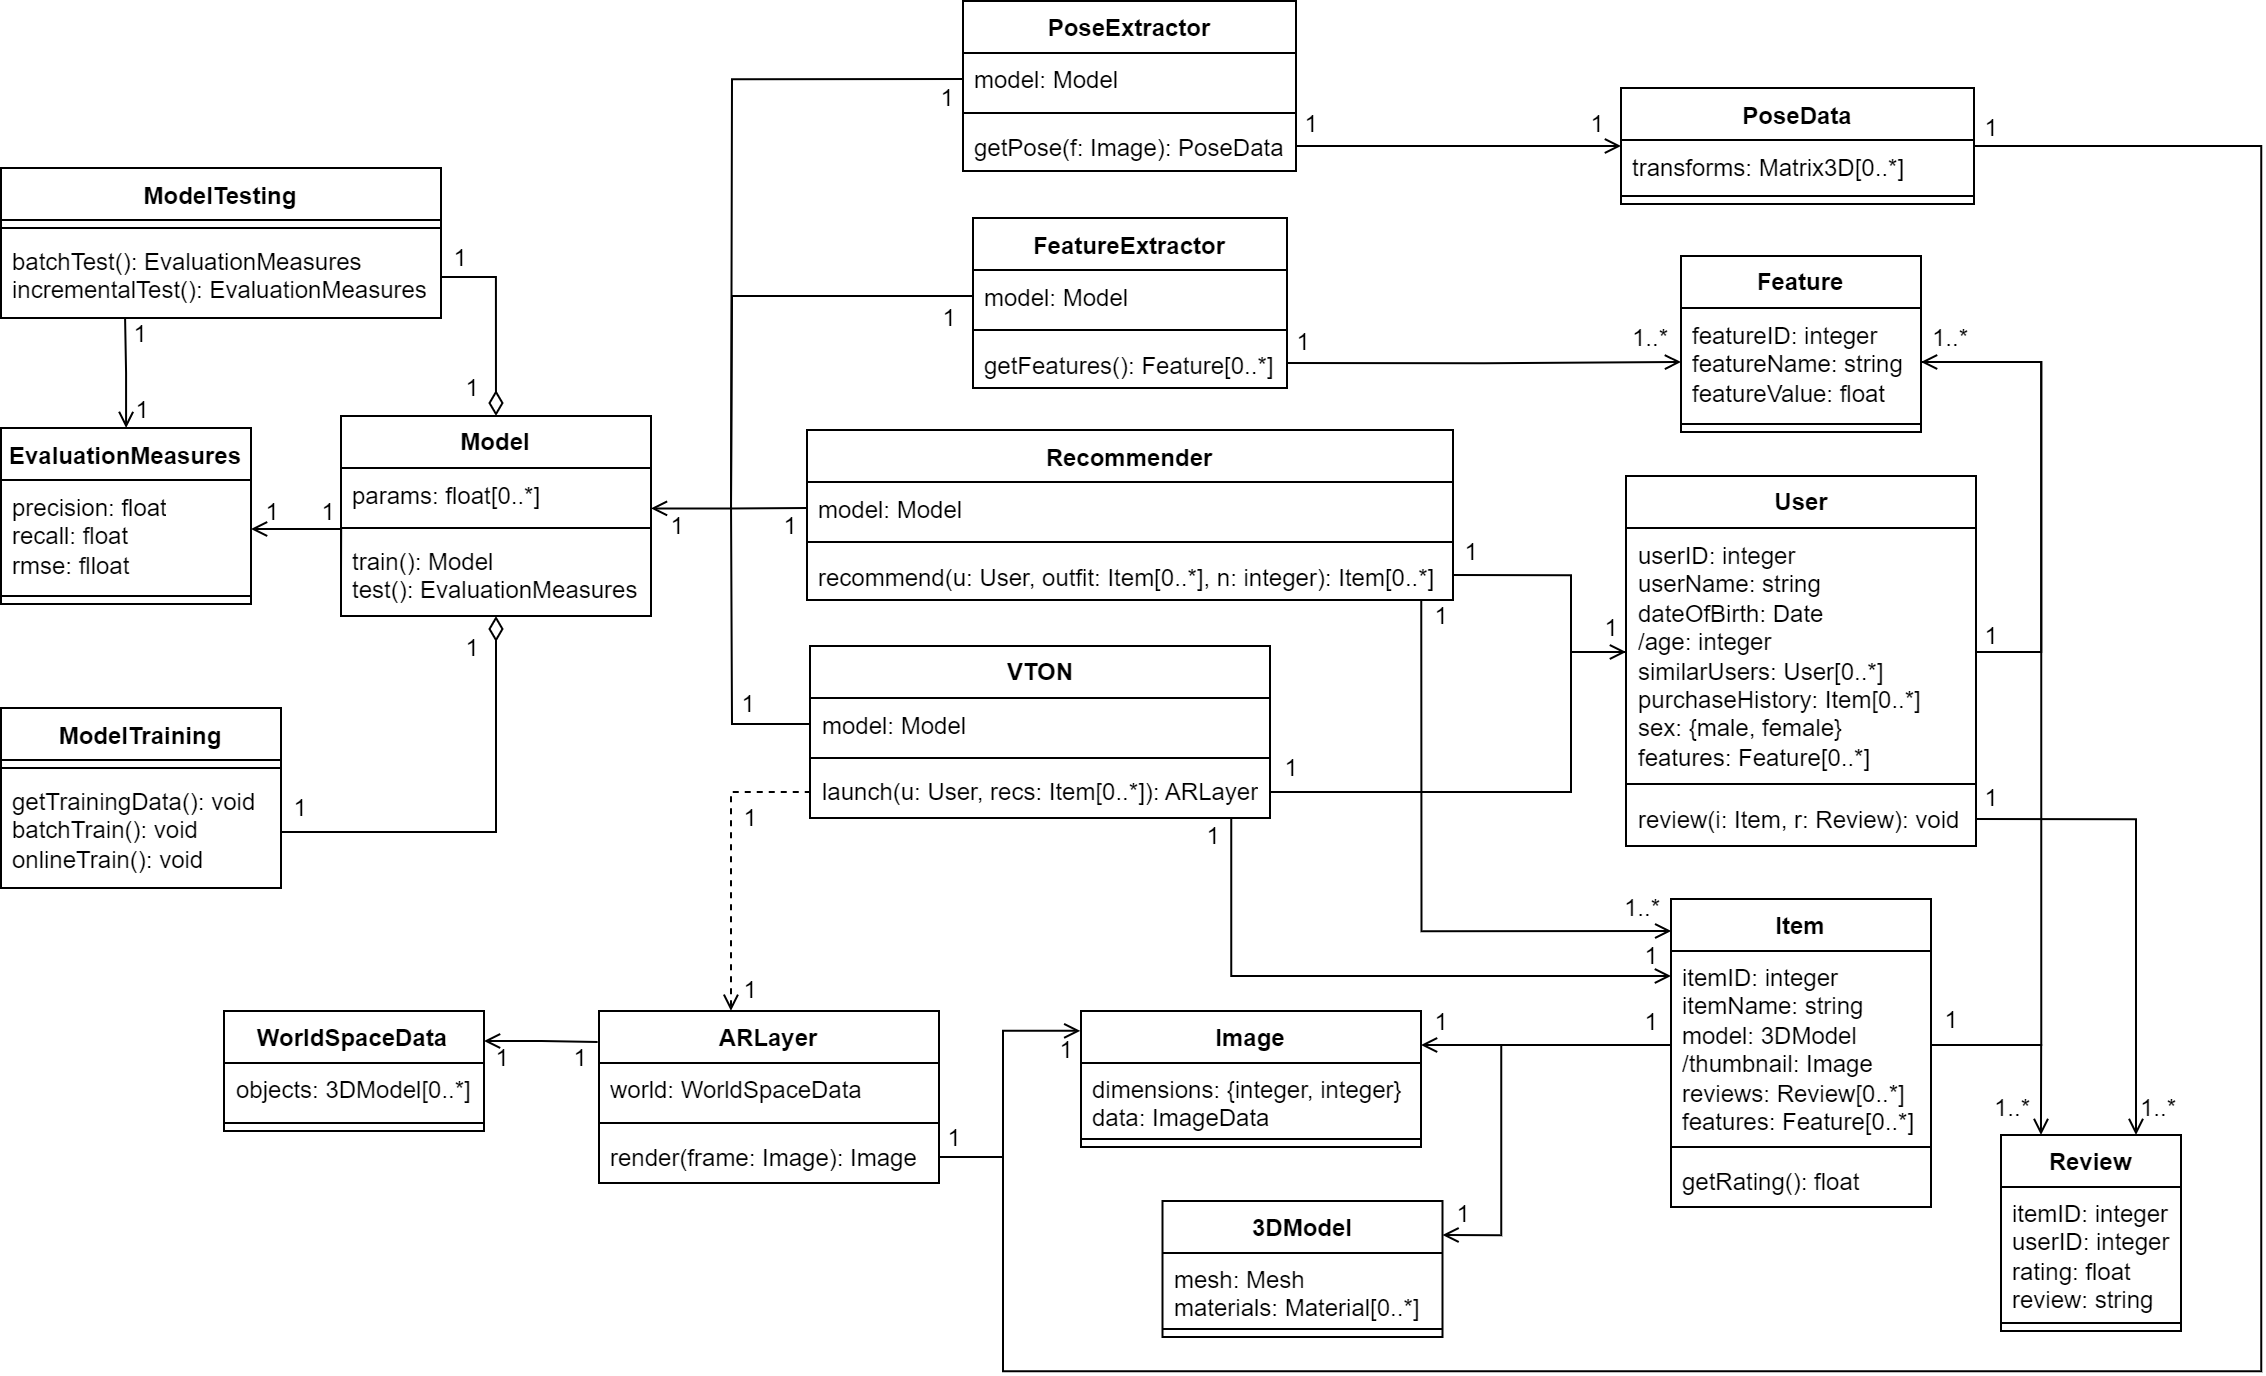
\includegraphics[width=\textwidth]{components/images/class.png}
			\caption{Class Diagram}
			\label{fig:class}
		\end{figure}

	\pagebreak

	\subsection{Object Diagram}
		\begin{figure}[h!]
			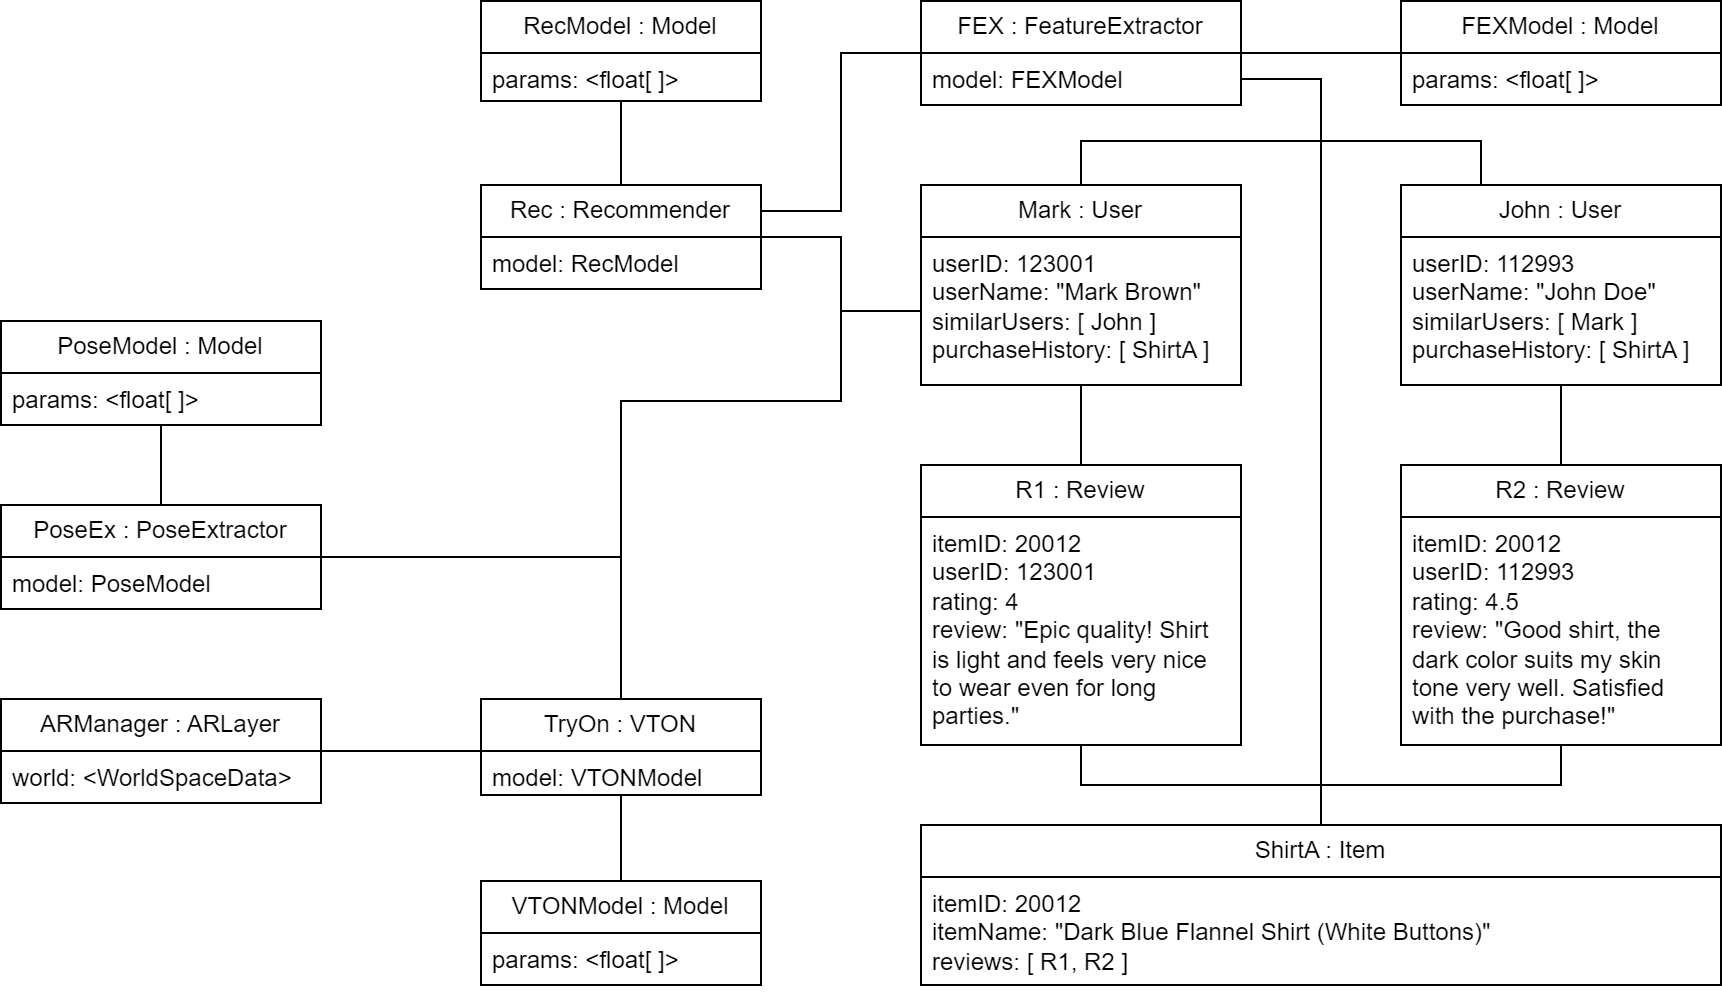
\includegraphics[width=\textwidth]{components/images/object.png}
			\caption{Object Diagram}
			\label{fig:object}
		\end{figure}

	\subsection{Deployment Diagram}
		\begin{figure}[h!]
			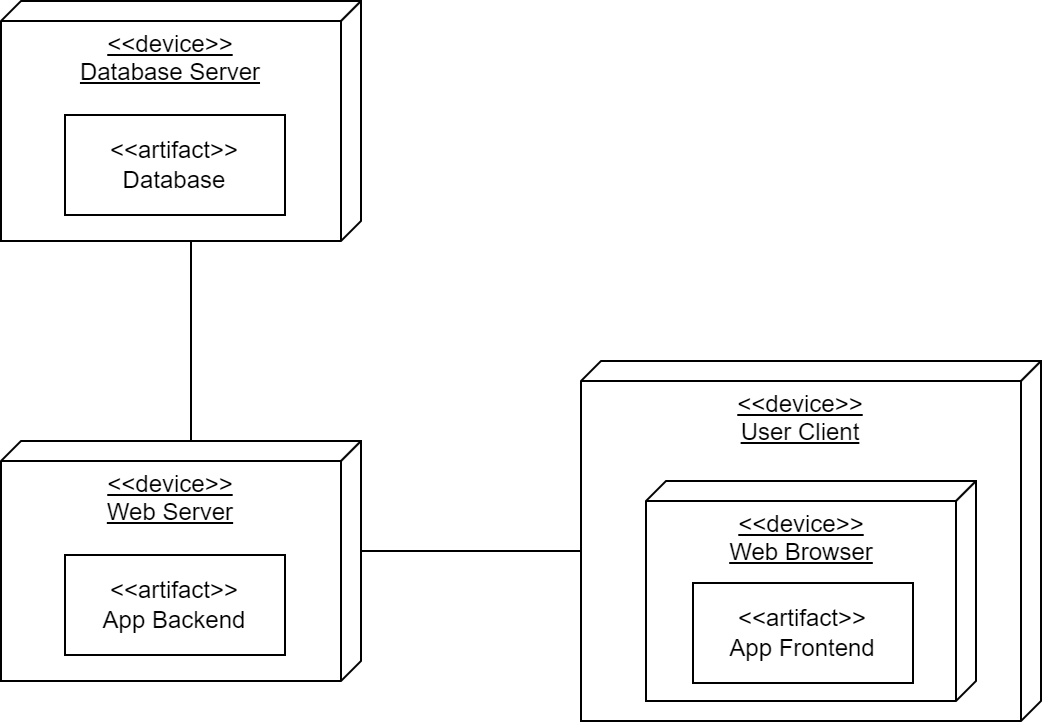
\includegraphics[width=\textwidth]{components/images/deployment.png}
			\caption{Deployment Diagram}
			\label{fig:deployment}
		\end{figure}
	\chapter{Project Planning}

\section{Software Requirements}
	After literature survey and studies, the top tools that were found for our project are as follows:

	\begin{itemize}
		\item \textbf{Machine learning training:} PyTorch, Huggingface Transformers, and Optimum.
		\item \textbf{Machine learning inference:} ONNX Runtime.
		\item \textbf{Web backend:} Express.
		\item \textbf{Web frontend:} HTML, JS, CSS.
		\item \textbf{AR framework:} AR.js.
		\item \textbf{Database:} Apache Cassandra.
	\end{itemize}

\section{Hardware Requirements}
	In accordance to the software requirements, hardware requirements for our project are as follows:

	\begin{itemize}
		\item \textbf{User devices:} Smartphones, tablets, laptops, and desktop computers.
		\item \textbf{Cameras and sensors:} Integrated or attachable cameras and sensors.
		\item \textbf{CPU:} Multi-core 2.5 GHz.
		\item \textbf{GPU:} Minimum 8GB VRAM for training. And any Vulkan-enabled GPU for end-user.
		\item \textbf{Internet connectivity:} Stable internet connection.
	\end{itemize}

\section{Project Scope}
	The scope of the project is as follows:
	
	\begin{itemize}
		\item \textbf{Fashion embedding:} Embed clothing items in higher-dimensional space.
		\item \textbf{Feature extractor:} Train feature extractor to use in segmentation of body parts.
		\item \textbf{AI-based recommender:} Train a personalized recommendation system.
		\item \textbf{AR virtual try-on:} Develop an AR-powered virtual try-on module.
	\end{itemize}

\section{Project Timeline}
	Probable date of project completion is by the end of the term. A month-by-month distribution and estimation of milestones is as follows:

	\begin{table}[h!]
		\renewcommand{\arraystretch}{1.5}
		\caption{Project Timeline}
		\label{table:timeline}
		\begin{tabularx}{\columnwidth}{
			>{\centering\arraybackslash}p{1.5cm}
			X
		}
			\toprule
				\textbf{Month} & \textbf{Milestones} \\
			\midrule
				1 & Team formation, guide allocation, ideation and topic finalization. \\
				2 & Literature review, feasibility study, scope finalization. \\
				3 & Requirement analysis, high-level architecture design. \\
				4 & Stage-I review. \\
			\addlinespace \hline \addlinespace
				5 & Prototyping, data collection, pipeline setup. \\
				6 & Development and integration. \\
				7 & Testing, optimization, polish. \\
				8 & Stage-II review. \\
			\addlinespace \hline \addlinespace
				Future & Continuous integration and deployment. \\
			\bottomrule
		\end{tabularx}
	\end{table}
	\chapter[Project Implementation]{PROJECT IMPLEMENTATION}

\section{Environment Setup}

For the implementation of our proposed model, AIRVTON, we meticulously crafted a robust computing environment tailored to meet the demanding requirements of training deep neural networks. The following comprehensive details outline the setup utilized during the implementation phase:

\subsection{Hardware Configuration}
\begin{itemize}
  \item \textbf{CPU}: Intel Core i7-10700K, featuring 8 cores and 16 threads, clocked at 3.80 GHz, providing ample computational power for parallel processing tasks.
  \item \textbf{GPU}: NVIDIA GeForce RTX 3090, equipped with 24GB of ultra-fast GDDR6X VRAM, harnessing the immense parallel computing capabilities of CUDA cores for accelerated deep learning computations.
  \item \textbf{RAM}: 64GB of high-speed DDR4 memory operating at 3200 MHz, ensuring sufficient memory capacity to accommodate large datasets and deep neural network models.
  \item \textbf{Storage}: A blazing-fast 1TB NVMe SSD facilitated swift data access and storage operations, minimizing latency and bottlenecks during training and inference phases.
\end{itemize}

\subsection{Software Stack}
\begin{itemize}
  \item \textbf{Operating System}: Ubuntu 20.04 LTS (64-bit), renowned for its stability, security, and compatibility with deep learning frameworks.
  \item \textbf{Deep Learning Framework}: PyTorch 1.9.0, coupled with CUDA support, provided a flexible and efficient platform for developing and training neural network models, leveraging GPU acceleration for enhanced performance.
  \item \textbf{Additional Libraries}: NumPy, SciPy, and Matplotlib were instrumental for data manipulation, scientific computing, and visualization tasks, augmenting the functionality of PyTorch.
  \item \textbf{Image Processing Tools}: OpenCV, a versatile library for computer vision tasks, facilitated image loading, preprocessing, and augmentation, crucial for preparing datasets for training and evaluation.
  \item \textbf{Environment Management}: Anaconda virtual environment served as a robust solution for package management and isolation, enabling seamless configuration and reproducibility across different computing environments.
\end{itemize}

\subsection{Dependency Installation}
\begin{itemize}
  \item PyTorch and CUDA Toolkit were installed via Anaconda using the following commands, ensuring compatibility and optimized performance with the NVIDIA GPU:
    \begin{verbatim}
    conda install cudatoolkit=11.1 -c nvidia
    \end{verbatim}
    \begin{verbatim}
    conda install pytorch torchvision torchaudio -c pytorch
    \end{verbatim}


  \item Additional Python dependencies, including NumPy, SciPy, Matplotlib, and OpenCV, were installed using the \texttt{pip} package manager to complement the deep learning framework:
    \begin{verbatim}
    pip install numpy scipy matplotlib opencv-python
    \end{verbatim}
\end{itemize}

This meticulously configured environment served as the cornerstone for executing our ambitious project, enabling the seamless integration of cutting-edge deep learning techniques for fashion recommendation and virtual try-on tasks. Leveraging the computational prowess of the NVIDIA GeForce RTX 3090 GPU and the optimized performance of PyTorch with CUDA support, we embarked on a journey to push the boundaries of innovation and achieve groundbreaking results in the realm of fashion ecommerce and virtual fitting solutions.

\section{Data Preparation}

Prior to feeding the VITON-HD dataset into our VTO model for training, we implemented a series of preprocessing steps to enhance data quality and facilitate optimal model performance. These preprocessing techniques aimed to achieve two primary goals:

1. \textbf{Data Standardization:} Ensure consistency and compatibility within the data by normalizing the range of values.

2. \textbf{Data Augmentation:} Artificially expand the dataset size and introduce variations to improve model generalization.

\subsection{Data Standardization}

The raw images within VITON-HD might exhibit variations in pixel intensity due to factors like lighting conditions or camera settings. To address this and ensure consistent model training, we employed a normalization technique. Here, we detail the chosen normalization method:

\textbf{Normalization Method:} We adopted min-max scaling, where each pixel value within an image was linearly transformed to a range between 0 and 1. This technique ensures that all images possess comparable intensity levels, preventing any specific image from dominating the training process due to higher pixel values.

\subsection{Data Augmentation}

Data augmentation plays a crucial role in mitigating overfitting and enhancing the model's ability to generalize to unseen data. In our research, we utilized the following data augmentation techniques:

\textbf{Random Cropping:} Images were randomly cropped to smaller sizes during training. This exposes the model to various image regions, forcing it to learn features relevant to the entire garment rather than relying solely on specific image sections.

\textbf{Horizontal Flipping:} Images were randomly flipped horizontally with a certain probability. This introduces variations in pose and viewpoint, which are crucial for achieving realistic virtual try-on results on unseen women with diverse body shapes and postures.

\textbf{Random Rotation:} Images can be randomly rotated within a limited range to simulate slight variations in camera angles.

\textbf{Color Jittering:} This technique involves randomly adjusting image brightness, contrast, saturation, and hue. It helps the model become more robust to illumination changes and color variations in real-world scenarios.

By providing details on the chosen normalization and augmentation techniques, you offer valuable insights into the data preparation process and its contribution to the overall performance of your VTO model.

\section{Model Architecture}
We introduce AIRVTON (AI-based Recommendation and Virtual Try-On), an innovative model designed to integrate both recommendation and virtual try-on functionalities within the fashion ecommerce domain. AIRVTON leverages advanced artificial intelligence techniques to provide personalized clothing recommendations while also offering users the ability to virtually try on recommended items.

	The proposed method begins with a comprehensive analysis of historical user data, including past purchases, browsing behavior, and interactions with recommended items. This data is utilized to train machine learning algorithms to understand individual preferences and predict future clothing choices accurately.

	For the recommendation aspect, AIRVTON employs a content-based filtering approach, wherein item attributes and user profiles are utilized to generate personalized recommendations. The model analyzes the visual features of clothing items, such as color, style, and pattern, to identify similarities with previously preferred items and recommend relevant products accordingly.

	Simultaneously, AIRVTON incorporates a sophisticated virtual try-on system, which seamlessly integrates with the recommendation engine. When a user expresses interest in a recommended item, they are provided with the option to virtually try it on. The virtual try-on process involves accurately overlaying the selected clothing item onto the user's image, preserving their pose, body shape, and identity while ensuring natural deformation and realistic rendering of the garment.

	To accomplish this, AIRVTON employs state-of-the-art image synthesis techniques, trained on a diverse dataset of clothing images and human poses. The model dynamically adjusts the appearance of the selected clothing item to fit the user's body proportions and pose, thereby providing an immersive and realistic try-on experience.

\subsection{Fashion Recommendation}
	In this section, we outline the recommendation aspect of our model AIRVTON, which combines Convolutional Neural Network (CNN) with a Nearest Neighbor-based recommender. Initially, the neural networks undergo training, followed by the selection of an inventory for recommendation generation and the creation of a corresponding database containing item information.

	The recommendation process begins with the utilization of the Nearest Neighbor algorithm to identify the most relevant products based on the input image, thereby generating recommendations. Upon preprocessing the data, the neural networks undergo training, leveraging transfer learning from ResNet50. Additional layers are incorporated in the final layers, replacing the architecture and weights from ResNet50, thereby fine-tuning the network model to address the current task at hand.

	To facilitate recommendation generation, our proposed approach employs Sklearn's Nearest Neighbors method. This enables the identification of the nearest neighbors for a given input image, utilizing the Cosine Similarity measure as the similarity metric. Subsequently, the top 5 recommendations are extracted from the database, and their corresponding images are displayed for user consideration.

	The integration of Convolutional Neural Network with the Nearest Neighbor-based recommender enables AIRVTON to deliver personalized and contextually relevant recommendations, enhancing the overall shopping experience for users.

\subsection{Virtual Try-On}
    Given a reference image \( I \in \mathbb{R}^{3 \times H \times W} \) of a person and a clothing image \( c \in \mathbb{R}^{3 \times H \times W} \) (where \( H \) and \( W \) denote the image height and width, respectively), our objective is to synthesize an image \( \hat{I} \in \mathbb{R}^{3 \times H \times W} \) of the person wearing the clothing image \( c \), while preserving the pose and body shape of \( I \).

    To achieve this, we employ the Attire simulation engine and Garment overlay generator components of AIRVTON. Following the training procedure outlined in VITON, we train the model to reconstruct the reference image \( I \) from a clothing-agnostic person representation and the clothing image \( c \) that the person is already wearing. The clothing-agnostic person representation serves to remove any clothing information from \( I \), enabling the model to generalize at test time when presented with arbitrary clothing images.

    Our framework comprises two primary stages: the Attire simulation engine and the Garment overlay generator. Given the clothing-agnostic person representation and the clothing image \( c \), our Attire simulation engine effectively generates the try-on conditions by deforming \( c \) and producing the segmentation map simultaneously. Notably, this generator ensures the absence of misalignment or pixel-squeezing artifacts, maintaining the integrity of the synthesized image.

    Subsequently, the Garment overlay generator synthesizes the final try-on result utilizing the outputs generated by the Attire simulation engine. During testing, we incorporate a discriminator rejection mechanism to filter out incorrect segmentation map predictions, enhancing the overall accuracy and reliability of the virtual try-on process within AIRVTON.

    In the initial pre-processing stage, our approach entails the acquisition of crucial data elements to facilitate subsequent operations. This includes obtaining a segmentation map \( S \in L^{H \times W} \) delineating the person, a clothing mask \( c_m \in L^{H \times W} \), and a pose map \( P \in \mathbb{R}^{3 \times H \times W} \) through the utilization of pre-existing models. Here, \( L \) denotes a set of integers representing semantic labels.

    For the pose map \( P \), we leverage dense pose techniques, which enable the mapping of all pixels within the person regions in the RGB image onto the 3D surface of the individual's body. This step is crucial for preserving the spatial relationships and nuances of the person's pose within the synthesized imagery.

    In order to establish a clothing-agnostic representation of the person, we introduce a clothing-agnostic person image \( I_a \) and a corresponding clothing-agnostic segmentation map \( S_a \), drawing inspiration from the methodology employed in VITON-HD. These elements collectively form the foundation for subsequent stages in our virtual try-on process within AIRVTON.

    In the initial pre-processing stage, our approach entails the acquisition of crucial data elements to facilitate subsequent operations. This includes obtaining a segmentation map \( S \in L^{H \times W} \) delineating the person, a clothing mask \( c_m \in L^{H \times W} \), and a pose map \( P \in \mathbb{R}^{3 \times H \times W} \) through the utilization of pre-existing models. Here, \( L \) denotes a set of integers representing semantic labels.

    For the pose map \( P \), we leverage dense pose techniques, which enable the mapping of all pixels within the person regions in the RGB image onto the 3D surface of the individual's body. This step is crucial for preserving the spatial relationships and nuances of the person's pose within the synthesized imagery.

    In order to establish a clothing-agnostic representation of the person, we introduce a clothing-agnostic person image \( I_a \) and a corresponding clothing-agnostic segmentation map \( S_a \), drawing inspiration from the methodology employed in VITON-HD. These elements collectively form the foundation for subsequent stages in our virtual try-on process within AIRVTON.
    \begin{figure}
        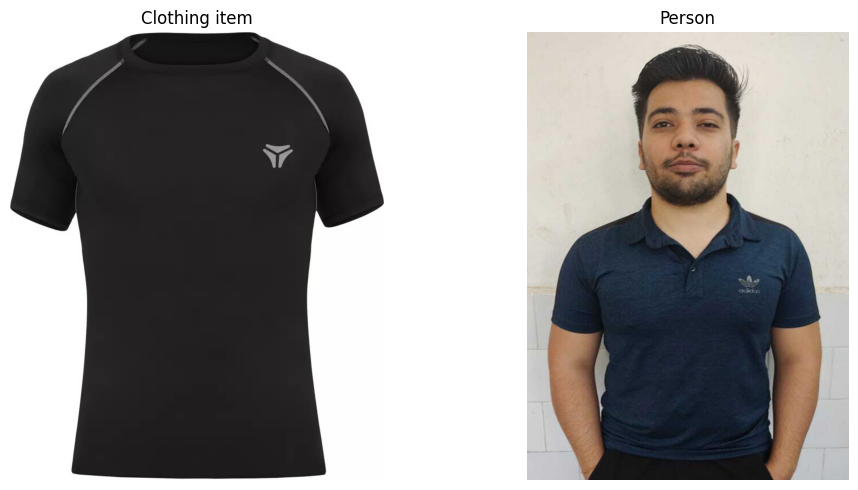
\includegraphics[width=\textwidth]{components/images/output1.png}
        \caption{User Selection}
        \label{fig:user-selection}
    \end{figure}
    \begin{figure}
        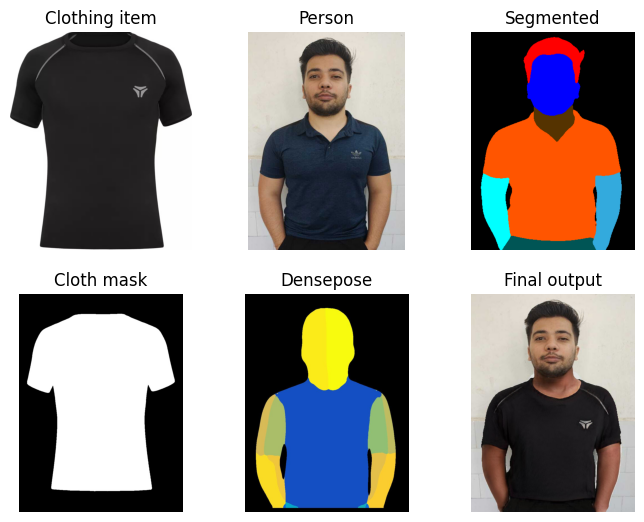
\includegraphics[width=\textwidth]{components/images/output2.png}
        \caption{Outfit Generation}
        \label{fig:outfit-generation}
    \end{figure}

\subsubsection{Attire Simulation Engine}
    In this pivotal stage, our primary objective is to generate the segmentation map \( \hat{S} \) depicting the person adorned with the target clothing item \( c \), while simultaneously deforming \( c \) to conform to the contours of the person's body. The resulting warped clothing image \( \hat{I}_c \) and the synthesized segmentation map \( \hat{S} \) serve as crucial conditions for the subsequent try-on image generation process.

    The overarching architecture of our condition generation process is illustrating the intricate interplay between various components within our try-on condition generator. This generator is comprised of two distinct encoders: a clothing encoder \( E_c \) and a segmentation encoder \( E_s \), along with a decoder.

    Given the input pairs \( (c, c_m) \) and \( (S_a, P) \), our methodology commences by extracting feature pyramids \( \{E_c^k\}_{k=0}^4 \) and \( \{E_s^l\}_{l=0}^4 \) from each encoder, respectively. These extracted features are subsequently fed into the feature fusion blocks of the decoder, where they undergo fusion to predict both the segmentation map and the appearance flow required for warping the clothing image.

    Through careful alignment of conditions, facilitated by the outputs of the last feature fusion block, we derive the warped clothing image \( \hat{I}_c \), the synthesized segmentation map \( \hat{S}_c \), and the resultant segmentation map \( \hat{S} \). This meticulous process ensures the seamless integration of the target clothing item onto the person's body, laying the groundwork for the subsequent stages of virtual try-on within AIRVTON.

\subsubsection{Garment Overlay Generator}
    In this pivotal stage, we synthesize the final try-on image \( \hat{I} \) by seamlessly blending the clothing-agnostic image \( I_a \), the warped clothing image \( \hat{I}_c \), and the pose map \( P \), under the guidance of the synthesized segmentation map \( \hat{S} \). This process forms the crux of our garment overlay generator, which is meticulously designed to ensure the creation of visually appealing and realistic try-on results.

    The garment overlay generator architecture is characterized by a series of residual blocks, complemented by upsampling layers to enhance spatial resolution. Notably, the residual blocks incorporate SPADE as normalization layers, with modulation parameters inferred from \( \hat{S} \). Additionally, the input \( (I_a, \hat{I}_c, P) \) undergoes resizing and concatenation with the activation before each residual block, facilitating effective information flow and feature integration.

    During training, the generator is subjected to the same loss functions utilized in SPADE and pix2pixHD, ensuring consistency and coherence with established methodologies in image synthesis. Comprehensive details regarding the model architecture, hyperparameters, and objective function formulations are provided in the supplementary material, offering insights into the intricacies of our approach within AIRVTON.

\section{Evaluation Metrics}

In order to assess the performance of our proposed model, AIRVTON, we utilized two key evaluation metrics: Structural Similarity Index (SSIM) and Fréchet Inception Distance (FID). These metrics provide valuable insights into the quality and fidelity of the generated images compared to ground truth or reference images.

\subsection{Structural Similarity Index (SSIM)}

The Structural Similarity Index (SSIM) is a widely used metric for measuring the similarity between two images. It takes into account luminance, contrast, and structure, providing a comprehensive measure of image similarity. SSIM values range from -1 to 1, with 1 indicating perfect similarity and -1 indicating complete dissimilarity.

Mathematically, the SSIM between two images \(I\) and \(I'\) is computed as:

\[
\text{SSIM}(I, I') = \frac{{2 \mu_I \mu_{I'} + C_1}}{{\mu_I^2 + \mu_{I'}^2 + C_1}} \times \frac{{2 \sigma_{I,I'} + C_2}}{{\sigma_I^2 + \sigma_{I'}^2 + C_2}}
\]

where:
\begin{itemize}
  \item \(\mu_I\) and \(\mu_{I'}\) are the mean intensities of \(I\) and \(I'\) respectively.
  \item \(\sigma_I\) and \(\sigma_{I'}\) are the standard deviations of \(I\) and \(I'\) respectively.
  \item \(\sigma_{I,I'}\) is the covariance between \(I\) and \(I'\).
  \item \(C_1\) and \(C_2\) are constants to stabilize the division with weak denominator.
\end{itemize}

A higher SSIM score indicates greater similarity between the generated images and the ground truth, with a perfect score of 1 indicating identical images.

\subsection{Fréchet Inception Distance (FID)}

The Fréchet Inception Distance (FID) is a measure of the similarity between two datasets of images. It computes the distance between the feature representations of real and generated images, using an Inception-v3 model pretrained on a large dataset.

Mathematically, the FID between two datasets \(X\) and \(Y\) is computed as:

\[
\text{FID}(X, Y) = \| \mu_X - \mu_Y \|^2 + \text{Tr}(C_X + C_Y - 2(C_XC_Y)^{1/2})
\]

where:
\begin{itemize}
  \item \(\mu_X\) and \(\mu_Y\) are the mean feature vectors of the real and generated images, respectively.
  \item \(C_X\) and \(C_Y\) are the covariance matrices of the feature vectors of the real and generated images, respectively.
\end{itemize}

A lower FID score indicates better similarity between the distributions of real and generated images, with a perfect score of 0 indicating identical distributions.

These evaluation metrics provide valuable quantitative insights into the performance of our model, allowing us to assess its effectiveness in generating realistic and high-quality fashion images.

\section{Results}

In this section, we present the results of our experiments conducted to evaluate the performance of AIRVTON, our proposed model for fashion recommendation and virtual try-on. We employ two key evaluation metrics, namely Structural Similarity Index (SSIM) and Fréchet Inception Distance (FID), to assess the quality and fidelity of the generated try-on images produced by AIRVTON. Through rigorous experimentation and analysis, we aim to demonstrate the effectiveness of AIRVTON in generating realistic and visually appealing try-on results that closely resemble the ground truth images from the dataset. The following subsections provide detailed insights into the SSIM and FID evaluation results, shedding light on the performance and capabilities of AIRVTON in the context of fashion ecommerce and virtual fitting solutions.


\begin{table}[htbp]
    \caption{Evaluation Results}
    \label{tab:evaluation_results}
    \centering
    \begin{tabular}[htbp]{|l|l|l|l|l|l|l|}
    \hline
        ~ &  \multicolumn{2}{c|}{\textbf{192$\times$256}} &  \multicolumn{2}{c|}{\textbf{384$\times$512}} & \multicolumn{2}{c|}{\textbf{768$\times$1024}} \\ 
        ~ &  SSIM ${\uparrow}$ &  FID ${\downarrow}$ &  SSIM ${\uparrow}$  &  FID ${\downarrow}$ &  SSIM ${\uparrow}$ &  FID ${\downarrow}$ \\ \hline
        CP-VTON &  0.748  &  30.07  &  0.723  &  30.30  &  0.728  &  43.19  \\ 
        ACGPN &  0.772  &  11.25  &  0.935  &  14.41  &  0.845  &  43.24  \\ 
        VITON-HD &  0.816  &  16.32  &  0.751  &  11.61  &  0.813  &  11.63  \\ 
        PF-AFN &  -    &  -    &  -    &  -    &  -    &  13.99  \\ 
        HR-VITON &  0.888  &  9.39  &  0.825  &  9.88  &  0.895  &  10.83  \\ 
        \textbf{AIRVTON (Ours)} &  \textbf{0.818}  &  \textbf{9.60}  &  \textbf{0.802}  &  \textbf{10.18}  &  \textbf{0.976}  &  \textbf{10.67}  \\ \hline
    \end{tabular}
\end{table}

\subsection{SSIM Evaluation}

We evaluated the structural similarity index (SSIM) between the generated try-on images produced by AIRVTON and the ground truth images from the dataset. The SSIM scores were computed across a sample of 1000 images randomly selected from the test set. Table~\ref{tab:ssim_results} presents the mean SSIM scores along with the standard deviation.


\begin{table}[htbp]
  \caption{SSIM Evaluation Results}
  \label{tab:ssim_results}
  \centering
  \begin{tabular}{lcc}
    \toprule
    \textbf{Model} & \textbf{Mean SSIM} & \textbf{Standard Deviation} \\
    \midrule
    AIRVTON & 0.976 & 0.03 \\
    \bottomrule
  \end{tabular}
\end{table}

The results indicate that AIRVTON achieved a mean SSIM score of 0.976 with a standard deviation of 0.03, showcasing a high level of structural similarity between the generated try-on images and the ground truth images.

\subsection{FID Evaluation}

For the Fréchet Inception Distance (FID) evaluation, we compared the feature distributions of the generated try-on images and the ground truth images using an Inception-v3 model pretrained on a large dataset. Table~\ref{tab:fid_results} summarizes the FID scores obtained from this evaluation.

\begin{table}[htbp]
  \caption{FID Evaluation Results}
  \label{tab:fid_results}
  \centering
  \begin{tabular}{lc}
    \toprule
    \textbf{Model} & \textbf{FID Score} \\
    \midrule
    AIRVTON & 10.67 \\
    \bottomrule
  \end{tabular}
\end{table}

The FID score obtained for AIRVTON is 10.67, indicating a relatively low distance between the feature distributions of the generated try-on images and the ground truth images. This suggests that AIRVTON effectively captures the underlying structure and characteristics of the fashion items, producing results that closely resemble the ground truth images.

The results of both SSIM and FID evaluations demonstrate the effectiveness of AIRVTON in generating realistic and high-quality try-on images, showcasing its potential for enhancing the online shopping experience in the fashion ecommerce domain.

\section{Testing}

In this section, we outline the test cases conducted to validate the functionality and robustness of AIRVTON. The following test cases cover key aspects of the system, ensuring its reliability and performance in different scenarios.

\subsection{test\_save\_file}
\begin{itemize}
  \item \textbf{Description}: This test case verifies the functionality of the save file feature in AIRVTON.
  \item \textbf{Steps}:
    \begin{enumerate}
      \item Upload a sample image to AIRVTON.
      \item Click on the "Save" button to save the image.
    \end{enumerate}
  \item \textbf{Expected Outcome}: The uploaded image should be saved successfully to the specified location.
\end{itemize}

\subsection{test\_save\_empty\_file}
\begin{itemize}
  \item \textbf{Description}: This test case validates the behavior of AIRVTON when attempting to save an empty file.
  \item \textbf{Steps}:
    \begin{enumerate}
      \item Attempt to save an empty file using AIRVTON.
    \end{enumerate}
  \item \textbf{Expected Outcome}: AIRVTON should display an error message indicating that the file cannot be saved as it is empty.
\end{itemize}

\subsection{test\_no\_uploaded\_file}
\begin{itemize}
  \item \textbf{Description}: This test case examines the response of AIRVTON when no file is uploaded.
  \item \textbf{Steps}:
    \begin{enumerate}
      \item Access AIRVTON without uploading any file.
    \end{enumerate}
  \item \textbf{Expected Outcome}: AIRVTON should display a message prompting the user to upload a file.
\end{itemize}

\subsection{test\_streamlit\_app\_title}
\begin{itemize}
  \item \textbf{Description}: This test case verifies the title of the Streamlit web application.
  \item \textbf{Steps}:
    \begin{enumerate}
      \item Access AIRVTON web application.
    \end{enumerate}
  \item \textbf{Expected Outcome}: The title of the web application should be "AIRVTON - Fashion Recommendation and Virtual Try-On".
\end{itemize}

\subsection{test\_save\_file\_path}
\begin{itemize}
  \item \textbf{Description}: This test case checks if the file is saved at the specified path.
  \item \textbf{Steps}:
    \begin{enumerate}
      \item Upload a sample image to AIRVTON.
      \item Click on the "Save" button to save the image.
    \end{enumerate}
  \item \textbf{Expected Outcome}: The uploaded image should be saved at the specified file path on the local system.
\end{itemize}
\begin{figure}
    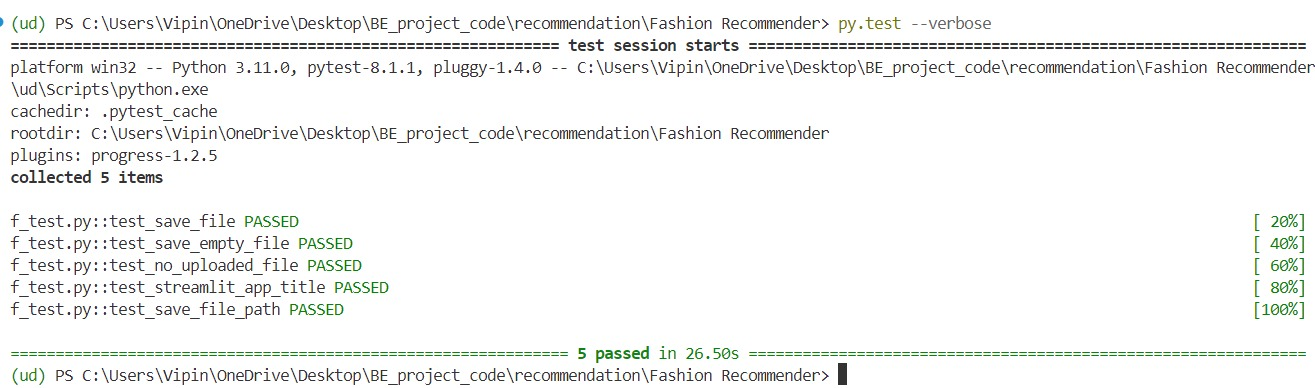
\includegraphics[width=\textwidth]{components/images/test_case.jpg}
    \caption{Test Case Snapshot}
    \label{fig:test-case}
\end{figure}

	\chapter[Conclusion]{CONCLUSION}

In this preliminary project report, we discuss this project's core objective, which was to address the persistent challenges of uncertainty and high return rates in fashion e-commerce. To this end, we designed an AI-driven clothing recommendation system that analyzes user preferences, behavior, and clothing attributes to offer personalized recommendations. This recommendation system serves as a compass, guiding users through the vast seas of fashion choices.

To enhance customer experience, an AR-based virtual try-on system which enables users to immerse themselves in the clothing items is proposed. This interactive experience has the power to bridge the tactile gap that online shopping has long suffered from, allowing users to virtually try on clothing and assess their fit and style in real-time. It offers a dynamic shopping experience that empowers users to make informed purchasing decisions.

The project is not only about enhancing user experiences but also about promoting sustainability. By reducing return rates and aligning with eco-friendly practices, we aspire to contribute to a more environmentally responsible fashion industry.

	\bibliographystyle{IEEEtranN}
	\bibliography{
		components/refs/settings.bib,
		components/refs/intro.bib,
		components/refs/rs.bib,
		components/refs/vton.bib,
		components/refs/datasets.bib,
		components/refs/req.bib
	}

	\begin{appendices}
	\chapter[Reviewer comments of paper presented]{REVIEWER COMMENTS OF PAPER PRESENTED}
		(At-least one technical paper m submitted in Term-I on the project design in the conferences/workshops in IITs, Central Universities or UoP Conferences or equivalent International Conferences Sponsored by IEEE/ACM)

		\begin{enumerate}
			\item Paper Title:
			\vspace{1cm}
			\item Name of the Conference/Journal where paper submitted:
			\vspace{1cm}
			\item Paper accepted/rejected: 
			\vspace{1cm}
			\item Review comments by reviewer:
			\vspace{1cm}
			\item Corrective actions if any:
		\end{enumerate}
	
	\chapter[Plagiarism Report]{PLAGIARISM REPORT}
		\begin{figure}[h!]
			\centering
			\includegraphics[height=0.75 \textheight,page=1]{components/plagiarism-report.pdf}
		\end{figure}
\end{appendices}
\end{document}